\chap{空间中的四元数}
\section{介绍}
在本章中,我们将展示如何使用四元数来围绕任意轴旋转向量。我们首先回顾了一些与四元数相关的历史,特别是本杰明·奥林德·罗德里格斯(Benjamin Olinde Rodrigues)的作用,他发现了旋转变换中半角的重要性。

对于特定的四元数积,当四元数表示为
$$
q=[\cos \theta, \sin \theta \mathbf{v}]
$$

一个向量围绕轴$\mathbf{v}$旋转一个角度$\theta$。但是,我们会发现,对于三重四元数的乘积,当四元数表示为
$$
q=\left[\cos \frac{1}{2} \theta, \sin \frac{1}{2} \theta \mathbf{v}\right]
$$

一个向量围绕轴$\mathbf{v}$旋转一个角度$\theta$。这种半角表示是罗德里格斯发现的。

关于组合代数的简短部分揭示了四元数是相当特殊的,并告诉我们为什么 Hamilton 不能识别基于超复数$z=s+ i+ bj $的代数。

然后,我们检查了各种四元数乘积,以发现它们的旋转性质。这从两个正交四元数开始,然后转向使用三重$q p q^{-1}$的一般情况,其中$q$是一个单位范数四元数,$p$是一个纯四元数。

本章介绍了两种将四元数乘积表示为矩阵的方法,这两种方法依次编码特征向量和特征值。最后,我们研究如何插值四元数。

我们继续将四元数表示为有序对,用斜体小写字母表示四元数,用粗体小写字母表示向量。

\section{一点历史}
本杰明·罗德里格斯(Benjamin Olinde Rodrigues, 1795-1851)出生于法国波尔多。他在巴黎学习,并于1816年获得博士学位,时年21岁。他论文的主题是求解 Legendre 多项式, Rodrigues 提出了一个解,这个解至今仍被称为 Rodrigues 公式。

虽然他从事政治和银行业,但他的博士研究证实他不仅仅是一个“娱乐”数学家,因为在1840年,他在《纯数学年鉴》(Annales de Mathématiques Pures et Appliquées)上发表了一篇关于变换群[20]的数学论文。该文包含了一个公式,其描述了一个几何结构,即两个连续的围绕不同的轴的旋转,等价于第三个围绕另一个轴的旋转。今天,我们知道这种对应称为Euler-Rodrigues参数化。欧拉在1775年已经证明了一次旋转可以表示围绕不同轴的两次连续旋转,但没有提供代数解。

如果我们将一个关于轴向量$\mathbf{a}$的旋转$\alpha$表示为$\mathbf{R}_{\alpha, \mathbf{a}}$,那么Rodrigues提供了一个解决方案
$$
\mathbf{R}_{\gamma, \mathbf{n}}=\mathbf{R}_{\alpha, \mathbf{l}} \mathbf{R}_{\beta, \mathbf{m}}
$$

形式为
\begin{align}
& \cos \frac{1}{2} \gamma=\cos \frac{1}{2} \alpha \cos \frac{1}{2} \beta-\sin \frac{1}{2} \alpha \sin \frac{1}{2} \beta \mathbf{l} \cdot \mathbf{m} \\
& \sin \frac{1}{2} \gamma \mathbf{n}=\sin \frac{1}{2} \alpha \cos \frac{1}{2} \beta \mathbf{l}+\cos \frac{1}{2} \alpha \sin \frac{1}{2} \beta \mathbf{m}+\sin \frac{1}{2} \alpha \sin \frac{1}{2} \beta \mathbf{l} \times \mathbf{m} .
\end{align}

Rodrigues没有使用(7.1)和(7.2)中使用的向量符号,因为这还没有被Hamilton定义,但他确实使用了这些向量积的代数等价物。图$7.1$显示了罗德里格斯使用的由轴和旋转角组成的球形三角形。

\begin{figure}[h!]
    \centering
    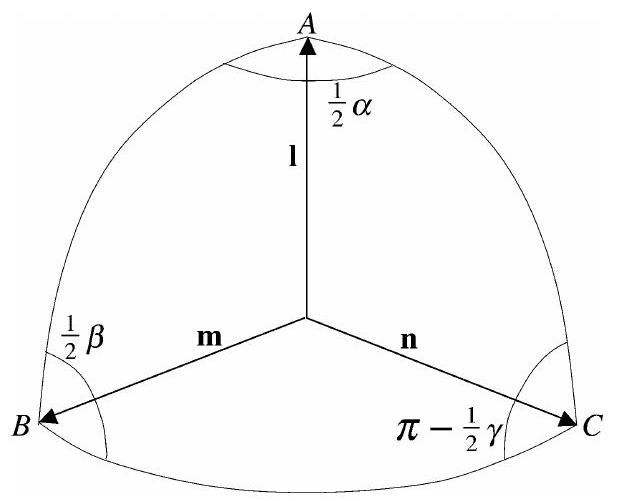
\includegraphics[max width=0.5\textwidth]{2023_01_16_a848224efad29cd66460g-105}
    \caption[short]{显示$\mathbf{l}$、$\mathbf{m}$和$\mathbf{n}$的Rodrigues球面三角形}
\end{figure}

式(7.1)和式(7.2)包含了一些四元数乘积所熟悉的特征,这些特征在下面的分析中变得很明显。我们从定义四元数开始

$$
\begin{aligned}
q_{l} & =\left[\cos \frac{1}{2} \alpha, \sin \frac{1}{2} \alpha \mathbf{l}\right] \\
q_{m} & =\left[\cos \frac{1}{2} \beta, \sin \frac{1}{2} \beta \mathbf{m}\right] \\
q_{n} & =\left[\cos \frac{1}{2} \gamma, \sin \frac{1}{2} \gamma \mathbf{n}\right]
\end{aligned}
$$

且乘积形式为
\begin{align}
q_{n}  =& q_{l} q_{m} \notag\\
=& \left[\cos \frac{1}{2} \alpha, \sin \frac{1}{2} \alpha \mathbf{l}\right]\left[\cos \frac{1}{2} \beta, \sin \frac{1}{2} \beta \mathbf{m}\right] \notag\\
=& \left[\cos \frac{1}{2} \alpha \cos \frac{1}{2} \beta-\sin \frac{1}{2} \alpha \sin \frac{1}{2} \beta \mathbf{l} \cdot \mathbf{m},\right. \notag\\
& \left.\sin \frac{1}{2} \alpha \cos \frac{1}{2} \beta \mathbf{l}+\cos \frac{1}{2} \alpha \sin \frac{1}{2} \beta \mathbf{m}+\sin \frac{1}{2} \alpha \sin \frac{1}{2} \beta \mathbf{l} \times \mathbf{m}\right] \notag\\
\cos \frac{1}{2} \gamma = & \cos \frac{1}{2} \alpha \cos \frac{1}{2} \beta-\sin \frac{1}{2} \alpha \sin \frac{1}{2} \beta \mathbf{l} \cdot \mathbf{m} \\
\sin \frac{1}{2} \gamma \mathbf{n} =& \sin \frac{1}{2} \alpha \cos \frac{1}{2} \beta \mathbf{l}+\cos \frac{1}{2} \alpha \sin \frac{1}{2} \beta \mathbf{m}+\sin \frac{1}{2} \alpha \sin \frac{1}{2} \beta \mathbf{l} \times \mathbf{m}
\end{align}

其中(7.3)和(7.4)分别与(7.1)和(7.2)相同。虽然Rodrigues没有发明四元数的形式
$$
q=s+a i+b j+c k,
$$

他在 Hamilton 之前就发现了四元数积的系数。这就是生活!\footnote{译注,法语:C'est la vie!}

Hamilton 在1843年10月发明了四元数,同年12月,他的朋友、爱尔兰数学家约翰·托马斯·格雷夫斯(John Thomas Graves, 1806-1870)发明了八度音阶,最终被称为八元数。英国数学家亚瑟·凯利(Arthur Cayley, 1821-1895)也对 Hamilton 的四元数很感兴趣,并于1845年独立发明了八元数。八元数最终被称为Cayley数而不是八元数,只是因为Graves直到1848年才发表了他的结果——比Cayley晚了3年!

正如四元数可以用复数的有序对来定义一样,八度或八元数也可以用四元数的有序对来定义。

\subsection{组合代数}
当一个特定的定律构成一个代数的基础时,它被称为组合代数。例如,我们知道在普通算术中
$$
a^{2} b^{2}=(a b)^{2} \qquad a, b \in \mathbb{R}
$$
比如
$$
3^{2} 4^{2}=12^{2}
$$
其中平方定律就是组合定律。

我们在第四章中发现,对于两个复数:
$$
\begin{aligned}
\left|z_{1}\right|\left|z_{2}\right| & =\left|z_{1} z_{2}\right| \qquad z_{1}, z_{2} \in \mathbb{C} \\
\left|z_{1}\right|^{2}\left|z_{2}\right|^{2} & =\left|z_{1} z_{2}\right|^{2} .
\end{aligned}
$$
举个例子, 给出
$$
\begin{aligned}
& z_{1}=a_{1}+b_{1} i \\
& z_{2}=a_{2}+b_{2} i
\end{aligned}
$$
然后
$$
\left(a_{1}^{2}+b_{1}^{2}\right)\left(a_{2}^{2}+b_{2}^{2}\right)=\left(a_{1} a_{2}-b_{1} b_{2}\right)^{2}+\left(a_{1} b_{2}+a_{2} b_{1}\right)^{2}
$$
这是一个2平方定律。

在第5章中,我们注意到对于两个四元数:
$$
\left|q_{a}\right|^{2}\left|q_{b}\right|^{2}=\left|q_{a} q_{b}\right|^{2} \quad q_{a}, q_{b} \in \mathbb{H} .
$$
举个例子, 给出
$$
\begin{aligned}
q_{a} & =\left[s_{a}, x_{a} \mathbf{i}+y_{a} \mathbf{j}+z_{a} \mathbf{k}\right] \\
q_{b} & =\left[s_{b}, x_{b} \mathbf{i}+y_{b} \mathbf{j}+z_{b} \mathbf{k}\right]
\end{aligned}
$$
然后
$$
\begin{aligned}
\left(s_{a}^{2}+x_{a}^{2}+y_{a}^{2}+z_{a}^{2}\right)\left(s_{b}^{2}+x_{b}^{2}+y_{b}^{2}+z_{b}^{2}\right)= & \left(s_{a} s_{b}-x_{a} x_{b}-y_{a} y_{b}-z_{a} z_{b}\right)^{2} \\
& +\left(s_{a} x_{b}+s_{b} x_{a}+y_{a} z_{b}-y_{b} z_{a}\right)^{2} \\
& +\left(s_{a} y_{b}+s_{b} y_{a}+z_{a} x_{b}-z_{b} x_{a}\right)^{2} \\
& +\left(s_{a} z_{b}+s_{b} z_{a}+x_{a} y_{b}-x_{b} y_{a}\right)^{2}
\end{aligned}
$$
这是四方定律。

除了复数,四元数在数学系统中占据着中心位置,今天有四个这样的组合代数:实$\mathbb{R}$、复$\mathbb{C}$、四元数$\mathbb{H}$和八元数$\mathbb{O}$,它们遵循$n$-平方的恒等式来计算它们的规范。1898年,德国数学家阿道夫·赫维茨(Adolf Hurwitz, 1859-1919)证明,只有当$n$等于1、2、4和8时,$n$的平方和与$n$的平方和的乘积才等于$n$的平方和,其中$n$用实数、复数、四元数和八元数表示。这就是所谓的“赫维茨定理”或“1,2,4,8定理”。没有其他系统是可能的,这表明四元数在数学领域是多么重要。因此,Hamilton对三元体系的探索是徒劳的,因为不存在三平方恒等式。

现在让我们研究如何使用四元数来围绕任意轴旋转向量。

\section{四元数乘积}
四元数$q$是标量$s$和向量$\mathbf{v}$的并集:
$$
q=[s, \mathbf{v}] \quad s \in \mathbb{R}, \mathbf{v} \in \mathbb{R}^{3}
$$

如果我们用$\mathbf{v}$的分量来表示它,我们有
$$
q=[s, x \mathbf{i}+y \mathbf{j}+z \mathbf{k}] \quad s, x, y, z \in \mathbb{R} .
$$

Hamilton曾希望四元数可以像复数转子一样使用,后者我们在第二章中看到了
$$
\mathbf{R}_{\theta}=\cos \theta+i \sin \theta
$$

将一个复数旋转$\theta$。单位范数四元数$q$可以用来旋转存储为纯四元数$p$的向量吗?是的,但只是在有限的意义上。为了理解这一点,让我们构造一个单位范数四元数$q$和一个纯四元数$p$的乘积。单位范数四元数$q$定义为
\begin{align}
\begin{aligned}
q & =[s, \lambda \hat{\mathbf{v}}] \quad s, \lambda \in \mathbb{R}, \hat{\mathbf{v}} \in \mathbb{R}^{3} \\
|\hat{\mathbf{v}}| & =1 \\
s^{2}+\lambda^{2} & =1
\end{aligned}
\end{align}
纯四元数$p$存储要旋转的向量$\mathbf{p}$:
$$
p=[0, \mathbf{p}] \quad \mathbf{p} \in \mathbb{R}^{3} .
$$

让我们计算乘积$p^{\prime}=q p$,并检查$p^{\prime}$的向量部分,看看$ \mathbf{p}$是否被旋转:
\begin{align}
\begin{aligned}
p^{\prime} & =q p \\
& =[s, \lambda \hat{\mathbf{v}}][0, \mathbf{p}] \\
& =[-\lambda \hat{\mathbf{v}} \cdot \mathbf{p}, s \mathbf{p}+\lambda \hat{\mathbf{v}} \times \mathbf{p}] .
\end{aligned}
\end{align}

我们可以从(7.6)中看到,结果是一个具有标量和向量分量的一般四元数。

\subsection{特殊情况}
上面提到的“狭义”是$\hat{\mathbf{v}}$必须垂直于$\mathbf{p}$,这使得点积项$-\lambda \hat{\mathbf{v}} \cdot \mathbf{p}$在(7.6)中消失,我们只剩下纯四元数
\begin{align}
    p^{\prime}=[0, s \mathbf{p}+\lambda \hat{\mathbf{v}} \times \mathbf{p}] .
\end{align}

图$7.2$说明了这种情况,其中$\mathbf{p}$垂直于$\hat{\mathbf{v}}$,而$\hat{\mathbf{v}} \times \mathbf{p}$垂直于包含$\mathbf{p}$和$\hat{\mathbf{v}}$的平面。现在因为$\hat{\mathbf{v}}$是一个单位向量,$|\mathbf{p}|=|\hat{\mathbf{v}} \times\mathbf{p}|$,这意味着我们有两个正交向量,即$\mathbf{p}$和$\hat{\mathbf{v}} \times\mathbf{p}$,它们的长度相同。因此,要绕$\hat{\mathbf{v}}$旋转$\mathbf{p}$,我们所要做的就是在(7.7)中使$s=\cos \theta$和$ \lambda=\sin \theta$:
$$
\begin{aligned}
p^{\prime} & =\left[0, \mathbf{p}^{\prime}\right] \\
& =[0, \cos \theta \mathbf{p}+\sin \theta \hat{\mathbf{v}} \times \mathbf{p}]
\end{aligned}
$$

\begin{figure}[h!]
    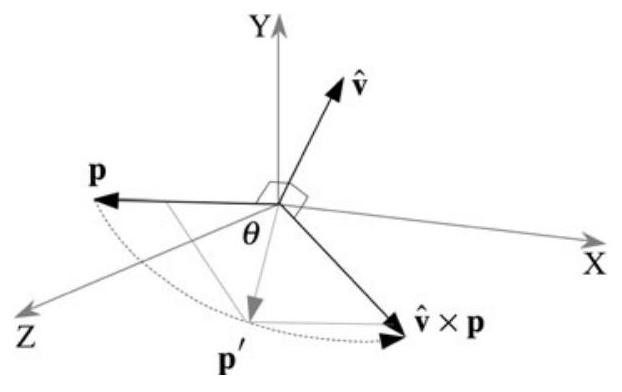
\includegraphics[max width=0.5\textwidth, center]{2023_01_16_a848224efad29cd66460g-109}
    \caption[short]{三个正交向量$\mathbf{p}, \hat{\mathbf{v}}$和$\hat{\mathbf{v}} \times \mathbf{p}$}
\end{figure}
\begin{figure}[h!]
    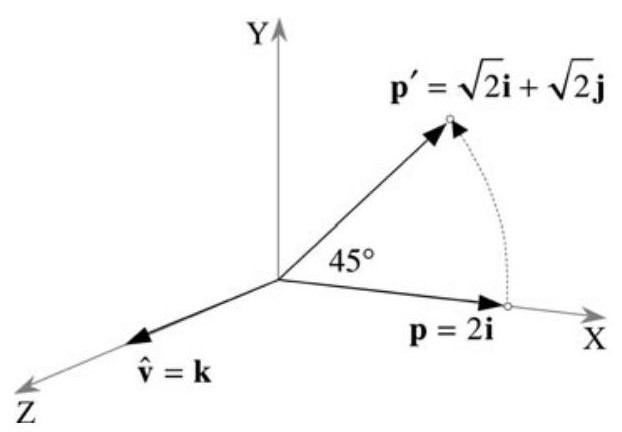
\includegraphics[max width=0.5\textwidth, center]{2023_01_16_a848224efad29cd66460g-109(1)}
    \caption[short]{向量$2 \mathbf{i}$被四元数$q=\left[\frac{\sqrt{2}}{2}, \frac{\sqrt{2}}{2} \mathbf{k}\right]$旋转$45^{\circ}$}
\end{figure}

例如,要绕$z$-轴旋转一个向量,$q$的向量$\hat{\mathbf{v}}$必须与$z$-轴对齐,如图7.3所示。如果我们使旋转角度$\theta=45^{\circ}$,那么
$$
\begin{aligned}
q & =[s, \lambda \hat{\mathbf{v}}] \\
& =[\cos \theta, \sin \theta \mathbf{k}] \\
& =\left[\frac{\sqrt{2}}{2}, \frac{\sqrt{2}}{2} \mathbf{k}\right]
\end{aligned}
$$
如果要旋转的向量是$\mathbf{p}=2 \mathbf{i}$,则
$$
\begin{aligned}
p & =[0, \mathbf{p}] \\
& =[0,2 \mathbf{i}] .
\end{aligned}
$$

现在有四个值得探索的乘积组合:$q p, pq, q^{-1} p$和$p q^{-1}$。不值得考虑$q p^{-1}$和$p^{-1} q$,因为$p^{-1}$只是颠倒了$\mathbf{p}$的方向。让我们从$q p$开始:
$$
\begin{aligned}
p^{\prime} & =q p \\
& =\left[\frac{\sqrt{2}}{2}, \frac{\sqrt{2}}{2} \mathbf{k}\right][0,2 \mathbf{i}] \\
& =\left[0,2 \frac{\sqrt{2}}{2} \mathbf{i}+2 \frac{\sqrt{2}}{2} \mathbf{k} \times \mathbf{i}\right] \\
& =[0, \sqrt{2} \mathbf{i}+\sqrt{2} \mathbf{j}]
\end{aligned}
$$
即$\mathbf{p}$已经被旋转$45^{\circ}$为$\mathbf{p}^{\prime}=\sqrt{2} \mathbf{i}+\sqrt{2} \mathbf{j}$。

接下来, $p q$ :
$$
\begin{aligned}
p^{\prime} & =p q \\
& =[0,2 \mathbf{i}]\left[\frac{\sqrt{2}}{2}, \frac{\sqrt{2}}{2} \mathbf{k}\right] \\
& =\left[0,2 \frac{\sqrt{2}}{2} \mathbf{i}-2 \frac{\sqrt{2}}{2} \mathbf{k} \times \mathbf{i}\right] \\
& =[0, \sqrt{2} \mathbf{i}-\sqrt{2} \mathbf{j}]
\end{aligned}
$$

即 $\mathbf{p}$ 已经被旋转 $-45^{\circ}$ 到 $\mathbf{p}^{\prime}=\sqrt{2} \mathbf{i}-\sqrt{2} \mathbf{j}$.

接下来,$q^{-1} p$,由于$q$是单位范数四元数,$q^{-1}=q^{*}$:
$$
\begin{aligned}
p^{\prime} & =q^{-1} p \\
& =\left[\frac{\sqrt{2}}{2},-\frac{\sqrt{2}}{2} \mathbf{k}\right][0,2 \mathbf{i}] \\
& =\left[0,2 \frac{\sqrt{2}}{2} \mathbf{i}-2 \frac{\sqrt{2}}{2} \mathbf{k} \times \mathbf{i}\right] \\
& =[0, \sqrt{2} \mathbf{i}-\sqrt{2} \mathbf{j}]
\end{aligned}
$$
即 $\mathbf{p}$ 已经被旋转 $-45^{\circ}$ 到 $\mathbf{p}^{\prime}=\sqrt{2} \mathbf{i}-\sqrt{2} \mathbf{j}$.

最后, $p q^{-1}$ :
$$
\begin{aligned}
p^{\prime} & =p q^{-1} \\
& =[0,2 \mathbf{i}]\left[\frac{\sqrt{2}}{2},-\frac{\sqrt{2}}{2} \mathbf{k}\right] \\
& =\left[0,2 \frac{\sqrt{2}}{2} \mathbf{i}+2 \frac{\sqrt{2}}{2} \mathbf{k} \times \mathbf{i}\right] \\
& =[0, \sqrt{2} \mathbf{i}+\sqrt{2} \mathbf{j}]
\end{aligned}
$$

即 $\mathbf{p}$ 已经被旋转 $45^{\circ}$ 到 $\mathbf{p}^{\prime}=\sqrt{2} \mathbf{i}+\sqrt{2} \mathbf{j}$. 因此,对于正交四元数,$\theta$是旋转角度,则
$$
\begin{aligned}
& q p=p q^{-1} \\
& p q=q^{-1} p
\end{aligned}
$$

\begin{figure}[h!]
    \centering
    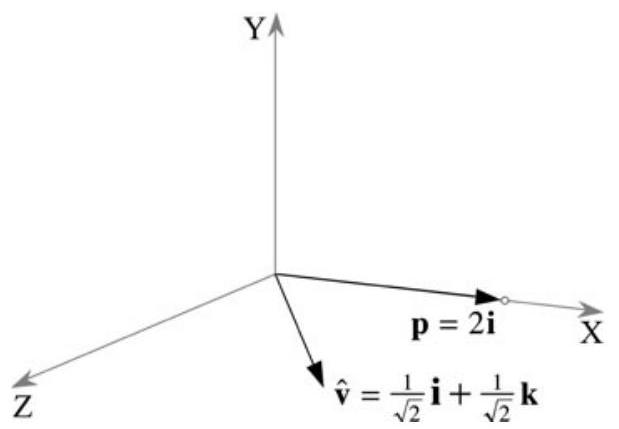
\includegraphics[max width=0.5\textwidth]{2023_01_16_a848224efad29cd66460g-111}
    \caption[short]{将向量$\mathbf{p}=2 \mathbf{i}$按四元数$q=[\cos \theta, \sin \theta \hat{\mathbf{v}}]$旋转}
\end{figure}

在继续之前,让我们看看当$\theta=180^{\circ}$时,乘积$q p$会发生什么变化:
$$
\begin{aligned}
p^{\prime} & =q p \\
& =[-1, \mathbf{0}][0,2 \mathbf{i}] \\
& =[0,-2 \mathbf{i}]
\end{aligned}
$$
即$\mathbf{p}$已被旋转$180^{\circ}$到$\mathbf{p}^{\prime}=-2 \mathbf{i}$。

注意,在上述所有乘积中,矢量在旋转过程中都没有缩放。这是因为$q$是一个单位范数四元数。现在让我们看看如果我们改变$\hat{\mathbf{v}}$和$\mathbf{p}$之间的角度会发生什么。让我们将角度减小到$45^{\circ}$,并保留$q$的单位向量,如图7.4所示。因此,
$$
\begin{aligned}
\hat{\mathbf{v}} & =\frac{1}{\sqrt{2}} \mathbf{i}+\frac{1}{\sqrt{2}} \mathbf{k} \\
q & =[\cos \theta, \sin \theta \hat{\mathbf{v}}] \\
p & =[0, \mathbf{p}] .
\end{aligned}
$$
这一次我们必须包含点积项$-\sin \theta \hat{\mathbf{v}} \cdot \mathbf{p}$,因为它不再是零:
\begin{align}
    \begin{aligned}
        p^{\prime} & =q p \\
        & =[\cos \theta, \sin \theta \hat{\mathbf{v}}][0, \mathbf{p}] \\
        & =[-\sin \theta \hat{\mathbf{v}} \cdot \mathbf{p}, \cos \theta \mathbf{p}+\sin \theta \hat{\mathbf{v}} \times \mathbf{p}] .
    \end{aligned}
\end{align}


将$\hat{\mathbf{v}}, \mathbf{p}$和$\theta=45^{\circ}$代入$(7.8)$,我们有
\begin{align}
    \begin{aligned}
        p^{\prime} & =\left[-\frac{\sqrt{2}}{2}\left(\frac{1}{\sqrt{2}} \mathbf{i}+\frac{1}{\sqrt{2}} \mathbf{k}\right) \cdot(2 \mathbf{i}), \frac{\sqrt{2}}{2} 2 \mathbf{i}+\frac{\sqrt{2}}{2}\left(\frac{1}{\sqrt{2}} \mathbf{i}+\frac{1}{\sqrt{2}} \mathbf{k}\right) \times 2 \mathbf{i}\right] \\
        & =[-1, \sqrt{2} \mathbf{i}+\mathbf{j}]
        \end{aligned}
\end{align}


不幸的是,它不再是纯四元数了。它没有被旋转$45^{\circ}$,并且向量的范数减少为$\sqrt{3}$ !向量乘以一个非正交四元数已将一些向量信息转换为四元数的标量分量。

\begin{figure}[h!]
    \centering
    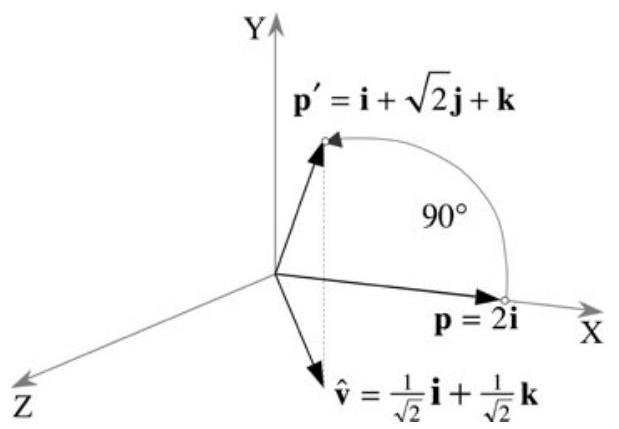
\includegraphics[max width=0.5\textwidth]{2023_01_16_a848224efad29cd66460g-112}
    \caption[short]{向量$2 \mathbf{i}$被旋转$90^{\circ}$为$\mathbf{i}+\sqrt{2} \mathbf{j}+\mathbf{k}$}
\end{figure}

\subsection{一般情况}
别担心。会不会是四元数逆运算用反了?让我们看看如果用$q^{-1}$后乘$q p$会发生什么。

给出
$$
q=\left[\cos \theta, \sin \theta\left(\frac{1}{\sqrt{2}} \mathbf{i}+\frac{1}{\sqrt{2}} \mathbf{k}\right)\right]
$$
接着
$$
\begin{aligned}
q^{-1} & =\left[\cos \theta,-\sin \theta\left(\frac{1}{\sqrt{2}} \mathbf{i}+\frac{1}{\sqrt{2}} \mathbf{k}\right)\right] \\
& =\left[\frac{\sqrt{2}}{2}, \frac{\sqrt{2}}{2}\left(\frac{1}{\sqrt{2}} \mathbf{i}+\frac{1}{\sqrt{2}} \mathbf{k}\right)\right] \\
& =\frac{1}{2}[\sqrt{2},-\mathbf{i}-\mathbf{k}] .
\end{aligned}
$$
因此,将(7.9)乘以$q^{-1}$,得到
\begin{align}
    \begin{aligned}
        q p q^{-1} & =[-1, \sqrt{2} \mathbf{i}+\mathbf{j}] \frac{1}{2}[\sqrt{2},-\mathbf{i}-\mathbf{k}] \\
        & =\frac{1}{2}[-\sqrt{2}-(\sqrt{2} \mathbf{i}+\mathbf{j}) \cdot(-\mathbf{i}-\mathbf{k}), \mathbf{i}+\mathbf{k}+\sqrt{2}(\sqrt{2} \mathbf{i}+\mathbf{j})-\mathbf{i}+\sqrt{2} \mathbf{j}+\mathbf{k}] \\
        & =\frac{1}{2}[-\sqrt{2}+\sqrt{2}, \mathbf{i}+\mathbf{k}+2 \mathbf{i}+\sqrt{2} \mathbf{j}-\mathbf{i}+\sqrt{2} \mathbf{j}+\mathbf{k}] \\
        & =[0, \mathbf{i}+\sqrt{2} \mathbf{j}+\mathbf{k}]
    \end{aligned}
\end{align}
这是一个纯四元数。此外,没有缩放,因为它的范数仍然是2,但向量已经旋转了$90^{\circ}$,而不是$45^{\circ}$,是所需角度的两倍,如图7.5所示。

如果以$q$和$q^{-1}$的纯四元数形式“夹”向量是正确的,那么将$\theta$增加到$90^{\circ}$应该将$ \mathbf{p}=2 \mathbf{i}$旋转$180^{\circ}$到$2 \mathbf{k}$。让我们试试这个。

令$\theta=90^{\circ}$,因此,
$$
\begin{aligned}
q p & =\left[0, \frac{1}{\sqrt{2}} \mathbf{i}+\frac{1}{\sqrt{2}} \mathbf{k}\right][0,2 \mathbf{i}] \\
& =\left[-\frac{2}{\sqrt{2}}, \frac{2}{\sqrt{2}} \mathbf{j}\right]
\end{aligned}
$$
接下来,我们将$q p$后乘$q^{-1}$:
$$
\begin{aligned}
q u p q^{-1} & =\left[-\frac{2}{\sqrt{2}}, \frac{2}{\sqrt{2}} \mathbf{j}\right]\left[0,-\frac{1}{\sqrt{2}} \mathbf{i}-\frac{1}{\sqrt{2}} \mathbf{k}\right] \\
& =[0, \mathbf{i}+\mathbf{k}-\mathbf{i}+\mathbf{k}] \\
& =[0,2 \mathbf{k}]
\end{aligned}
$$
这证实了我们的预测,并表明$q p q^{-1}$可行。现在我们来看看这个两倍角是如何产生的。首先定义一个单位范数四元数$q$:
$$
q=[s, \lambda \hat{\mathbf{v}}]
$$
其中$s^{2}+\lambda^{2}=1$。要旋转的向量$\mathbf{p}$被编码为纯四元数:
$$
p=[0, \mathbf{p}]
$$
且这个四元数的逆$q^{-1}$是
$$
q^{-1}=[s,-\lambda \hat{\mathbf{v}}]
$$
因此,积$q p q^{-1}$为
$$
\begin{aligned}
q p q^{-1}= & {[s, \lambda \hat{\mathbf{v}}][0, \mathbf{p}][s,-\lambda \hat{\mathbf{v}}] } \\
= & {[-\lambda \hat{\mathbf{v}} \cdot \mathbf{p}, s \mathbf{p}+\lambda \hat{\mathbf{v}} \times \mathbf{p}][s,-\lambda \hat{\mathbf{v}}] } \\
= & {\left[-\lambda s \hat{\mathbf{v}} \cdot \mathbf{p}+\lambda s \mathbf{p} \cdot \hat{\mathbf{v}}+\lambda^{2}(\hat{\mathbf{v}} \times \mathbf{p}) \cdot \hat{\mathbf{v}}\right.} \\
& \lambda^{2}(\hat{\mathbf{v}} \cdot \mathbf{p}) \hat{\mathbf{v}}+s^{2} \mathbf{p}+\lambda s \hat{\mathbf{v}} \times \mathbf{p} \\
& \left.-\lambda s \mathbf{p} \times \hat{\mathbf{v}}-\lambda^{2}(\hat{\mathbf{v}} \times \mathbf{p}) \times \hat{\mathbf{v}}\right] \\
= & {\left[\lambda^{2}(\hat{\mathbf{v}} \times \mathbf{p}) \cdot \hat{\mathbf{v}}, \lambda^{2}(\hat{\mathbf{v}} \cdot \mathbf{p}) \hat{\mathbf{v}}+s^{2} \mathbf{p}+2 \lambda s \hat{\mathbf{v}} \times \mathbf{p}-\lambda^{2}(\hat{\mathbf{v}} \times \mathbf{p}) \times \hat{\mathbf{v}}\right] }
\end{aligned}
$$
请注意,
$$
(\hat{\mathbf{v}} \times \mathbf{p}) \cdot \hat{\mathbf{v}}=0
$$
且
$$
(\hat{\mathbf{v}} \times \mathbf{p}) \times \hat{\mathbf{v}}=(\hat{\mathbf{v}} \cdot \hat{\mathbf{v}}) \mathbf{p}-(\mathbf{p} \cdot \hat{\mathbf{v}}) \hat{\mathbf{v}}=\mathbf{p}-(\mathbf{p} \cdot \hat{\mathbf{v}}) \hat{\mathbf{v}}
$$
因此,
\begin{align}
\begin{aligned}
q p q^{-1} & =\left[0, \lambda^{2}(\hat{\mathbf{v}} \cdot \mathbf{p}) \hat{\mathbf{v}}+s^{2} \mathbf{p}+2 \lambda s \hat{\mathbf{v}} \times \mathbf{p}-\lambda^{2} \mathbf{p}+\lambda^{2}(\mathbf{p} \cdot \hat{\mathbf{v}}) \hat{\mathbf{v}}\right] \\
& =\left[0,2 \lambda^{2}(\hat{\mathbf{v}} \cdot \mathbf{p}) \hat{\mathbf{v}}+\left(s^{2}-\lambda^{2}\right) \mathbf{p}+2 \lambda s \hat{\mathbf{v}} \times \mathbf{p}\right]
\end{aligned}
\end{align}
显然,这是一个纯四元数,因为标量分量为零。然而,角度翻倍的来源并不明显。但是看看当我们令$s=\cos \theta$和$\lambda=\sin \theta$时,会发生什么:
$$
\begin{aligned}
q p q^{-1} & =\left[0,2 \sin ^{2} \theta(\hat{\mathbf{v}} \cdot \mathbf{p}) \hat{\mathbf{v}}+\left(\cos ^{2} \theta-\sin ^{2} \theta\right) \mathbf{p}+2 \sin \theta \cos \theta \hat{\mathbf{v}} \times \mathbf{p}\right] \\
& =[0,(1-\cos 2 \theta)(\hat{\mathbf{v}} \cdot \mathbf{p}) \hat{\mathbf{v}}+\cos 2 \theta \mathbf{p}+\sin 2 \theta \hat{\mathbf{v}} \times \mathbf{p}] .
\end{aligned}
$$
双倍角度项出现了!现在,如果我们想让这个乘积实际旋转向量$\theta$,那么我们必须从一开始就把$\theta$减半到$q$:
\begin{align}
    q=\left[\cos \frac{1}{2} \theta, \sin \frac{1}{2} \theta \hat{\mathbf{v}}\right]
\end{align}
这使得
\begin{align}
q p q^{-1}=[0,(1-\cos \theta)(\hat{\mathbf{v}} \cdot \mathbf{p}) \hat{\mathbf{v}}+\cos \theta \mathbf{p}+\sin \theta \hat{\mathbf{v}} \times \mathbf{p}]
\end{align}
积$q p q^{-1}$是Hamilton发现的,但他没有发表结果。Cayley也发现了这种乘积,并于1845年发表了结果。然而,Altmann指出,“在Cayley的文集中,他承认Hamilton优先”[2],这是一个很好的姿态。然而,在Hamilton和Cayley之前认识到半角参数重要性的人是rodrigues,他发表了一个Hamilton没有看到的解决方案,但显然是Cayley看到的。

让我们使用前面的例子来测试(7.13),其中我们围绕四元数$\hat{\mathbf{v}}=(1 / \sqrt{2}) \mathbf{i}+(1 / \sqrt{2}) \mathbf{k}$旋转一个向量$\mathbf{p}=2 \mathbf{i}$, $\theta=90^{\circ}$
$$
\begin{aligned}
q u p q^{-1} & =[0,(1-\cos \theta)(\hat{\mathbf{v}} \cdot \mathbf{p}) \hat{\mathbf{v}}+\cos \theta \mathbf{p}+\sin \theta \hat{\mathbf{v}} \times \mathbf{p}] \\
& =[0,(\hat{\mathbf{v}} \cdot \mathbf{p}) \hat{\mathbf{v}}+\hat{\mathbf{v}} \times \mathbf{p}] \\
& =\left[0, \frac{2}{\sqrt{2}}\left(\frac{1}{\sqrt{2}} \mathbf{i}+\frac{1}{\sqrt{2}} \mathbf{k}\right)+\sqrt{2} \mathbf{j}\right] \\
& =[0, \mathbf{i}+\sqrt{2} \mathbf{j}+\mathbf{k}]
\end{aligned}
$$
这与(7.10)一致。因此,当单位范数四元数采用如下形式时
$$
q=\left[\cos \frac{1}{2} \theta, \sin \frac{1}{2} \theta \hat{\mathbf{v}}\right]
$$
存储待旋转向量的纯四元数采用这种形式
$$
p=[0, \mathbf{p}]
$$
纯四元数
$$
p^{\prime}=q p q^{-1}
$$
存储旋转后的向量$\mathbf{p}^{\prime}$。我们来看看为什么这个乘积保留了旋转矢量的大小。
$$
\begin{aligned}
\left|p^{\prime}\right| & =|q p|\left|q^{-1}\right| \\
& =|q||p|\left|q^{-1}\right| \\
& =|q|^{2}|p|
\end{aligned}
$$
且如果$q$是一个单位范数四元数,$|q|=1$,则$\left|p^{\prime}\right|=|p|$。

你可能想知道,如果乘积颠倒到$q^{-1} p q$会发生什么?一种猜测是旋转顺序颠倒了,但让我们看看代数分析证实了什么。
$$
\begin{aligned}
q^{-1} p q= & {[s,-\lambda \hat{\mathbf{v}}][0, \mathbf{p}][s, \lambda \hat{\mathbf{v}}] } \\
= & {[\lambda \hat{\mathbf{v}} \cdot \mathbf{p}, s \mathbf{p}-\lambda \hat{\mathbf{v}} \times \mathbf{p}][s, \lambda \hat{\mathbf{v}}] } \\
= & {[\lambda s \hat{\mathbf{v}} \cdot \mathbf{p}-\lambda s \mathbf{p} \cdot \hat{\mathbf{v}}} \\
& \left.\lambda^{2} \hat{\mathbf{v}} \times \mathbf{p} \cdot \hat{\mathbf{v}}+\lambda^{2} \hat{\mathbf{v}} \cdot \mathbf{p} \hat{\mathbf{v}}+s^{2} \mathbf{p}-\lambda s \hat{\mathbf{v}} \times \mathbf{p}+\lambda s \mathbf{p} \times \hat{\mathbf{v}}-\lambda^{2} \hat{\mathbf{v}} \times \mathbf{p} \times \hat{\mathbf{v}}\right] \\
= & {\left[\lambda^{2}(\hat{\mathbf{v}} \times \mathbf{p}) \cdot \hat{\mathbf{v}}, \lambda^{2}(\hat{\mathbf{v}} \cdot \mathbf{p}) \hat{\mathbf{v}}+s^{2} \mathbf{p}-2 \lambda s \hat{\mathbf{v}} \times \mathbf{p}-\lambda^{2}(\hat{\mathbf{v}} \times \mathbf{p}) \times \hat{\mathbf{v}}\right] }
\end{aligned}
$$
又一次
$$
(\hat{\mathbf{v}} \times \mathbf{p}) \cdot \hat{\mathbf{v}}=0
$$
且
$$
(\hat{\mathbf{v}} \times \mathbf{p}) \times \hat{\mathbf{v}}=\mathbf{p}-(\mathbf{p} \cdot \hat{\mathbf{v}}) \hat{\mathbf{v}}
$$
因此,
$$
\begin{aligned}
q^{-1} p q & =\left[0, \lambda^{2}(\hat{\mathbf{v}} \cdot \mathbf{p}) \hat{\mathbf{v}}+s^{2} \mathbf{p}-2 \lambda s \hat{\mathbf{v}} \times \mathbf{p}-\lambda^{2} \mathbf{p}+\lambda^{2}(\mathbf{p} \cdot \hat{\mathbf{v}}) \hat{\mathbf{v}}\right] \\
& =\left[0,2 \lambda^{2}(\hat{\mathbf{v}} \cdot \mathbf{p}) \hat{\mathbf{v}}+\left(s^{2}-\lambda^{2}\right) \mathbf{p}-2 \lambda s \hat{\mathbf{v}} \times \mathbf{p}\right]
\end{aligned}
$$
再次,让我们令$s=\cos \theta$和$\lambda=\sin \theta$:
$$
q^{-1} p q=[0,(1-\cos 2 \theta)(\hat{\mathbf{v}} \cdot \mathbf{p}) \hat{\mathbf{v}}+\cos 2 \theta \mathbf{p}-\sin 2 \theta \hat{\mathbf{v}} \times \mathbf{p}]
$$
则唯一改变$q p q^{-1}$的是叉乘项的符号,叉乘项的方向是相反的。但是,我们必须记住通过将$\theta$减半来补偿角度加倍:
\begin{align}
q^{-1} p q=[0,(1-\cos \theta)(\hat{\mathbf{v}} \cdot \mathbf{p}) \hat{\mathbf{v}}+\cos \theta \mathbf{p}-\sin \theta \hat{\mathbf{v}} \times \mathbf{p}]
\end{align}
让我们看看当我们使用(7.14)绕四元数的向量$\hat{\mathbf{v}}=(1 / \sqrt{2}) \mathbf{i}+(1 / \sqrt{2}) \mathbf{k}$旋转$\mathbf{p}=2 \mathbf{i}, 90^{\circ}$会发生什么:
$$
\begin{aligned}
q^{-1} p q & =\left[0, \frac{2}{\sqrt{2}}\left(\frac{1}{\sqrt{2}} \mathbf{i}+\frac{1}{\sqrt{2}} \mathbf{k}\right)-\sqrt{2} \mathbf{j}\right] \\
& =[0, \mathbf{i}-\sqrt{2} \mathbf{j}+\mathbf{k}]
\end{aligned}
$$
它将$\mathbf{p}$绕四元数的向量顺时针旋转$90^{\circ}$。因此,转子$q p q^{-1}$逆时针旋转一个向量,$q^{-1} p q$顺时针旋转一个向量:
$$
\begin{aligned}
q p q^{-1} & =[0,(1-\cos \theta)(\hat{\mathbf{v}} \cdot \mathbf{p}) \hat{\mathbf{v}}+\cos \theta \mathbf{p}+\sin \theta \hat{\mathbf{v}} \times \mathbf{p}] \\
q^{-1} p q & =[0,(1-\cos \theta)(\hat{\mathbf{v}} \cdot \mathbf{p}) \hat{\mathbf{v}}+\cos \theta \mathbf{p}-\sin \theta \hat{\mathbf{v}} \times \mathbf{p}]
\end{aligned}
$$

\begin{figure}[h!]
    \centering
    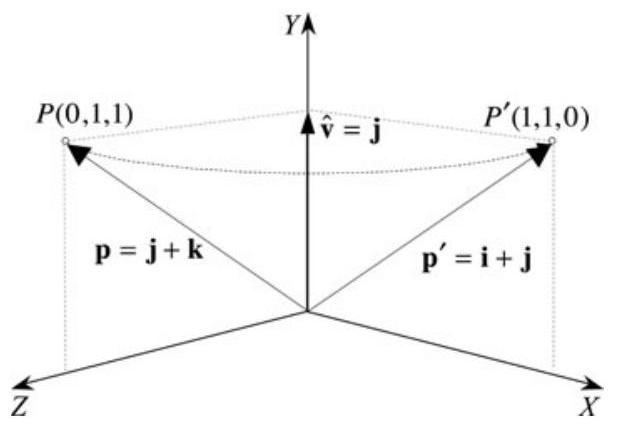
\includegraphics[max width=0.5\textwidth]{2023_01_16_a848224efad29cd66460g-116}
    \caption[short]{点$P(0,1,1)$围绕$y$轴旋转$90^{\circ}$到$P^{\prime}(1,1,0)$}
\end{figure}

让我们计算另一个例子。考虑图$7.6$中的点$P(0,1,1)$,它将围绕$y$轴旋转$90^{\circ}$。我们可以看到旋转后的点$P^{\prime}$的坐标为$(1,1,0)$,我们将用代数方法确认。点$P$在纯四元数中由它的位置向量$\mathbf{P}$表示
$$
p=[0, \mathbf{p}] \text {. }
$$
旋转轴为$\hat{\mathbf{v}}=\mathbf{j}$,要旋转的向量为$\mathbf{p}=\mathbf{j}+\mathbf{k}$。因此,
$$
\begin{aligned}
\operatorname{qpq}^{-1} & =[0,(1-\cos \theta)(\hat{\mathbf{v}} \cdot \mathbf{p}) \hat{\mathbf{v}}+\cos \theta \mathbf{p}+\sin \theta \hat{\mathbf{v}} \times \mathbf{p}] \\
& =[0, \mathbf{j} \cdot(\mathbf{j}+\mathbf{k}) \mathbf{j}+\mathbf{j} \times(\mathbf{j}+\mathbf{k})] \\
& =[0, \mathbf{i}+\mathbf{j}]
\end{aligned}
$$
且确认$P$确实被旋转到$(1,1,0)$。

现在我们来研究一下这个乘积是如何用矩阵形式表示的。

\section{矩阵形式的四元数}
在发现了一个向量方程来表示三重$q p q^{-1}$之后,让我们继续把它转换成一个矩阵。我们将探讨两种方法:第一种是简单的向量方法,它将表示$q p q^{-1}$的向量方程直接转换为矩阵形式。第二种方法使用矩阵代数来开发一个相当巧妙的解决方案。

\subsection{向量方法}
对于向量法,将单位范数四元数描述为
$$
\begin{aligned}
q & =[s, \mathbf{v}] \\
& =[s, x \mathbf{i}+y \mathbf{j}+z \mathbf{k}]
\end{aligned}
$$
其中
$$
s^{2}+|\mathbf{v}|^{2}=1
$$
而纯四元数为
$$
\begin{aligned}
p & =[0, \mathbf{p}] \\
& =\left[0, x_{p} \mathbf{i}+y_{p} \mathbf{j}+z_{p} \mathbf{k}\right] .
\end{aligned}
$$
计算$q p q^{-1}$的简单方法是使用(7.11)并将$|\mathbf{v}|$替换为$\lambda$:
$$
\begin{aligned}
q p q^{-1} & =\left[0,2 \lambda^{2}(\hat{\mathbf{v}} \cdot \mathbf{p}) \hat{\mathbf{v}}+\left(s^{2}-\lambda^{2}\right) \mathbf{p}+2 \lambda s \hat{\mathbf{v}} \times \mathbf{p}\right] \\
& =\left[0,2|\mathbf{v}|^{2}(\hat{\mathbf{v}} \cdot \mathbf{p}) \hat{\mathbf{v}}+\left(s^{2}-|\mathbf{v}|^{2}\right) \mathbf{p}+2|\mathbf{v}| s \hat{\mathbf{v}} \times \mathbf{p}\right]
\end{aligned}
$$
接下来,我们用$\mathbf{v}$替换$|\mathbf{v}| \hat{\mathbf{v}}$:
$$
q p q^{-1}=\left[0,2(\mathbf{v} \cdot \mathbf{p}) \mathbf{v}+\left(s^{2}-|\mathbf{v}|^{2}\right) \mathbf{p}+2 s \mathbf{v} \times \mathbf{p}\right]
$$
最后,由于我们在工作中使用的是单位规范的四元数,以防止缩放。
$$
s^{2}+|\mathbf{v}|^{2}=1
$$
且
$$
s^{2}-|\mathbf{v}|^{2}=2 s^{2}-1
$$
因此,
$$
q p q^{-1}=\left[0,2(\mathbf{v} \cdot \mathbf{p}) \mathbf{v}+\left(2 s^{2}-1\right) \mathbf{p}+2 s \mathbf{v} \times \mathbf{p}\right]
$$
如果我们令$p^{\prime}=q p q^{-1}$,这是一个纯四元数,我们有
$$
\begin{aligned}
p^{\prime} & =q p q^{-1} \\
& =\left[0, \mathbf{p}^{\prime}\right] \\
& =\left[0,2(\mathbf{v} \cdot \mathbf{p}) \mathbf{v}+\left(2 s^{2}-1\right) \mathbf{p}+2 s \mathbf{v} \times \mathbf{p}\right] \\
\mathbf{p}^{\prime} & =2(\mathbf{v} \cdot \mathbf{p}) \mathbf{v}+\left(2 s^{2}-1\right) \mathbf{p}+2 s \mathbf{v} \times \mathbf{p} .
\end{aligned}
$$
我们只对旋转向量$\mathbf{p}^{\prime}$感兴趣,它由三个项$2(\mathbf{v} \cdot \mathbf{p}) \mathbf{v}$, $\left(2s ^{2}-1\right) \mathbf{p}$和$ 2s \mathbf{v} \times \mathbf{p}$组成,它们可以由三个单独的矩阵表示并求和。
$$
\begin{aligned}
2(\mathbf{v} \cdot \mathbf{p}) \mathbf{v} & =2\left(x x_{p}+y y_{p}+z z_{p}\right)(x \mathbf{i}+y \mathbf{j}+z \mathbf{k}) \\
& =\left[\begin{array}{lll}
2 x^{2} & 2 x y & 2 x z \\
2 x y & 2 y^{2} & 2 y z \\
2 x z & 2 y z & 2 z^{2}
\end{array}\right]\left[\begin{array}{l}
x_{p} \\
y_{p} \\
z_{p}
\end{array}\right] \\
\end{aligned}
$$

$$
\begin{aligned}
\left(2 s^{2}-1\right) \mathbf{p} & =\left(2 s^{2}-1\right) x_{p} \mathbf{i}+\left(2 s^{2}-1\right) y_{p} \mathbf{j}+\left(2 s^{2}-1\right) z_{p} \mathbf{k} \\
& =\left[\begin{array}{ccc}
2 s^{2}-1 & 0 & 0 \\
0 & 2 s^{2}-1 & 0 \\
0 & 0 & 2 s^{2}-1
\end{array}\right]\left[\begin{array}{l}
x_{p} \\
y_{p} \\
z_{p}
\end{array}\right]\\
2 s \mathbf{v} \times \mathbf{p} & =2 s\left(\left(y z_{p}-z y_{p}\right) \mathbf{i}+\left(z x_{p}-x z_{p}\right) \mathbf{j}+\left(x y_{p}-y x_{p}\right) \mathbf{k}\right) \\
& =\left[\begin{array}{ccc}
0 & -2 s z & 2 s y \\
2 s z & 0 & -2 s x \\
-2 s y & 2 s x & 0
\end{array}\right]\left[\begin{array}{l}
x_{p} \\
y_{p} \\
z_{p}
\end{array}\right] .
\end{aligned}
$$
把这些矩阵加起来:
\begin{align}
\mathbf{p}^{\prime}=\left[\begin{array}{ccc}
2\left(s^{2}+x^{2}\right)-1 & 2(x y-s z) & 2(x z+s y) \\
2(x y+s z) & 2\left(s^{2}+y^{2}\right)-1 & 2(y z-s x) \\
2(x z-s y) & 2(y z+s x) & 2\left(s^{2}+z^{2}\right)-1
\end{array}\right]\left[\begin{array}{l}
x_{p} \\
y_{p} \\
z_{p}
\end{array}\right]
\end{align}
或
\begin{align}
\mathbf{p}^{\prime}=\left[\begin{array}{ccc}
1-2\left(y^{2}+z^{2}\right) & 2(x y-s z) & 2(x z+s y) \\
2(x y+s z) & 1-2\left(x^{2}+z^{2}\right) & 2(y z-s x) \\
2(x z-s y) & 2(y z+s x) & 1-2\left(x^{2}+y^{2}\right)
\end{array}\right]\left[\begin{array}{l}
x_{p} \\
y_{p} \\
z_{p}
\end{array}\right]
\end{align}
其中
$$
\left[0, \mathbf{p}^{\prime}\right]=q p q^{-1}
$$
现在让我们反转乘积。要计算$q^{-1} p q$的向量部分,我们所要做的就是将$2s \mathbf{v} \times\mathbf{p}$的符号颠倒:
\begin{align}
\mathbf{p}^{\prime}=\left[\begin{array}{ccc}
2\left(s^{2}+x^{2}\right)-1 & 2(x y+s z) & 2(x z-s y) \\
2(x y-s z) & 2\left(s^{2}+y^{2}\right)-1 & 2(y z+s x) \\
2(x z+s y) & 2(y z-s x) & 2\left(s^{2}+z^{2}\right)-1
\end{array}\right]\left[\begin{array}{l}
x_{p} \\
y_{p} \\
z_{p}
\end{array}\right]
\end{align}
或
\begin{align}
\mathbf{p}^{\prime}=\left[\begin{array}{ccc}
1-2\left(y^{2}+z^{2}\right) & 2(x y+s z) & 2(x z-s y) \\
2(x y-s z) & 1-2\left(x^{2}+z^{2}\right) & 2(y z+s x) \\
2(x z+s y) & 2(y z-s x) & 1-2\left(x^{2}+y^{2}\right)
\end{array}\right]\left[\begin{array}{l}
x_{p} \\
y_{p} \\
z_{p}
\end{array}\right]
\end{align}
其中
$$
\left[0, \mathbf{p}^{\prime}\right]=q^{-1} p q .
$$
观察出(7.17)是(7.15)的转置,(7.18)是(7.16)的转置。

\subsection{矩阵方法}
$$
\begin{aligned}
q_{a} & =\left[s_{a}, x_{a} \mathbf{i}+y_{a} \mathbf{j}+z_{a} \mathbf{k}\right] \\
q_{b} & =\left[s_{b}, x_{b} \mathbf{i}+y_{b} \mathbf{j}+z_{b} \mathbf{k}\right]
\end{aligned}
$$
它们的乘积是
$$
\begin{aligned}
q_{a} q_{b}=&\left[s_{a}, x_{a} \mathbf{i}+y_{a} \mathbf{j}+z_{a} \mathbf{k}\right]\left[s_{b}, x_{b} \mathbf{i}+y_{b} \mathbf{j}+z_{b} \mathbf{k}\right] \\
=&\left[s_{a} s_{b}-x_{a} x_{b}-y_{a} y_{b}-z_{a} z_{b},\right. \\
& s_{a}\left(x_{b} \mathbf{i}+y_{b} \mathbf{j}+z_{b} \mathbf{k}\right) \\
& +s_{b}\left(x_{a} \mathbf{i}+y_{a} \mathbf{j}+z_{a} \mathbf{k}\right) \\
& \left.+\left(y_{a} z_{b}-y_{b} z_{a}\right) \mathbf{i}+\left(x_{b} z_{a}-x_{a} z_{b}\right) \mathbf{j}+\left(x_{a} y_{b}-x_{b} y_{a}\right) \mathbf{k}\right] \\
=&\left[s_{a} s_{b}-x_{a} x_{b}-y_{a} y_{b}-z_{a} z_{b}\right. \text {, } \\
& \left(s_{a} x_{b}+s_{b} x_{a}+y_{a} z_{b}-y_{b} z_{a}\right) \mathbf{i} \\
& +\left(s_{a} y_{b}+s_{b} y_{a}+x_{b} z_{a}-x_{a} z_{b}\right) \mathbf{j} \\
& \left.+\left(s_{a} z_{b}+s_{b} z_{a}+x_{a} y_{b}-x_{b} y_{a}\right) \mathbf{k}\right] \\
=&\begin{bmatrix}s_{a} & -x_{a} & -y_{a} & -z_{a} \\x_{a} & s_{a} & -z_{a} & y_{a} \\y_{a} & z_{a} & s_{a} & -x_{a} \\z_{a} & -y_{a} & x_{a} & s_{a}\end{bmatrix}\begin{bmatrix}s_{b} \\x_{b} \\y_{b} \\z_{b}\end{bmatrix}=\mathbf{A} q_{b} .
\end{aligned}
$$
在这个阶段,我们有四元数$q_{a}$表示为矩阵$\mathbf{A}$,四元数$q_{b}$表示为列向量。现在让我们在不改变结果的情况下,将$q_{b}$设为矩阵,$q_{a}$设为列向量:
$$
q_{a} q_{b}=\begin{bmatrix}
s_{b} & -x_{b} & -y_{b} & -z_{b} \\
x_{b} & s_{b} & z_{b} & -y_{b} \\
y_{b} & -z_{b} & s_{b} & x_{b} \\
z_{b} & y_{b} & -x_{b} & s_{b}
\end{bmatrix}\begin{bmatrix}
s_{a} \\
x_{a} \\
y_{a} \\
z_{a}
\end{bmatrix}=\mathbf{B} q_{a}
$$
现在我们有两种方法来计算$q_{a} q_{b}$,我们需要一种方法来区分这两个矩阵。设$\mathbf{L}$是保留从左到右四元数序列的矩阵,$\mathbf{R}$是将序列从右到左反转的矩阵:
$$
\begin{aligned}
& q_{a} q_{b}=\mathbf{L}\left(q_{a}\right) q_{b}= {\left[\begin{array}{cccc}
s_{a} & -x_{a} & -y_{a} & -z_{a} \\
x_{a} & s_{a} & -z_{a} & y_{a} \\
y_{a} & z_{a} & s_{a} & -x_{a} \\
z_{a} & -y_{a} & x_{a} & s_{a}
\end{array}\right]\left[\begin{array}{c}
s_{b} \\
x_{b} \\
y_{b} \\
z_{b}
\end{array}\right] } \\
\end{aligned}
$$
$$
\begin{aligned}
& q_{a} q_{b}=\mathbf{R}\left(q_{b}\right) q_{a}=\left[\begin{array}{cccc}
s_{b} & -x_{b} & -y_{b} & -z_{b} \\
x_{b} & s_{b} & z_{b} & -y_{b} \\
y_{b} & -z_{b} & s_{b} & x_{b} \\
z_{b} & y_{b} & -x_{b} & s_{b}
\end{array}\right]\left[\begin{array}{c}
s_{a} \\
x_{a} \\
y_{a} \\
z_{a}
\end{array}\right] .
\end{aligned}
$$
请记住$\mathbf{L}\left(q_{a}\right) q_{b}=\mathbf{R}\left(q_{b}\right) q_{a}$,因为这是理解下一阶段的核心。此外,如果你不能理解第一篇阅读中的论点,也不要感到惊讶。作者花了很多小时痛苦地试图破译原始算法,这个解释已经扩展,以确保您不会遭受同样的经历!

首先,让我们使用矩阵$\mathbf{L}$和$\mathbf{R}$将四元数积$q_{a} q_{c} q_{b}$重新排列到$q_{a} q_{b} q_{c}$,即将$q_{c}$从中间移到右边。我们从四元数积$q_{a} q_{c} q_{b}$开始,并将其分为$q_{a} q_{c}$和$q_{b}$两部分。我们可以这样做,因为四元数代数是符合结合律的:
$$
q_{a} q_{c} q_{b}=\left(q_{a} q_{c}\right) q_{b}
$$
前面已经演示过,可以用$\mathbf{L}\left(q_{a}\right) q_{c}$替换乘积$q_{a} q_{c}$
$$
q_{a} q_{c} q_{b}=\mathbf{L}\left(q_{a}\right) q_{c} q_{b}
$$
我们现在有另外两个部分:$\mathbf{L}\left(q_{a}\right) q_{c}$和$q_{b}$,它们可以使用$\mathbf{R}$来反转,而不会影响结果:
$$
q_{a} q_{c} q_{b}=\mathbf{L}\left(q_{a}\right) q_{c} q_{b}=\mathbf{R}\left(q_{b}\right) \mathbf{L}\left(q_{a}\right) q_{c}
$$
这样就实现了将$q_{c}$移到右边的目标。但最重要的结果是,矩阵$\mathbf{R}\left(q_{b}\right)$和$\mathbf{L}\left(q_{a}\right)$可以相乘,形成一个对$q_{c}$操作的矩阵。

现在让我们重复相同的过程来重新排列乘积$q p q^{-1}$。目标是将$p$从$q$和$q^{-1}$的中间移到右边。这样做的原因是将$q$和$q^{-1}$以两个矩阵的形式放在一起,它们可以相乘成一个矩阵。

我们从四元数积$q p q^{-1}$开始,并将其分为$q p$和$q^{-1}$两部分
$$
q p q^{-1}=(q p) q^{-1}
$$
乘积$ qp $可以替换为$\mathbf{L}(q) p$:
$$
q p q^{-1}=\mathbf{L}(q) p q^{-1}
$$
我们现在有另外两个部分:$\mathbf{L}(q) p$和$q^{-1}$,可以使用$\mathbf{R}$反转而不影响结果:
$$
q p q^{-1}=\mathbf{L}(q) p q^{-1}=\mathbf{R}\left(q^{-1}\right) \mathbf{L}(q) p
$$
这就实现了把p移到右边的目标。

下一步是计算$\mathbf{L}(q)$和$\mathbf{R}\left(q^{-1}\right)$使用$q=[s, x \mathbf{i}+y \mathbf{j}+z \mathbf{k}]$。

$\mathbf{L}(q)$很简单,因为它与$\mathbf{L}\left(q_{a}\right)$相同:
$$
\mathbf{L}(q)=\left[\begin{array}{cccc}
s & -x & -y & -z \\
x & s & -z & y \\
y & z & s & -x \\
z & -y & x & s
\end{array}\right]
$$
$\mathbf{R}\left(q^{-1}\right)$也很简单,但需要将原始定义中的$q_{b}$转换为$q^{-1}$,这是通过反转向量分量的符号来实现的:
$$
\mathbf{R}\left(q^{-1}\right)=\left[\begin{array}{cccc}
s & x & y & z \\
-x & s & -z & y \\
-y & z & s & -x \\
-z & -y & x & s
\end{array}\right]
$$

\begin{figure}[h!]
    \centering
    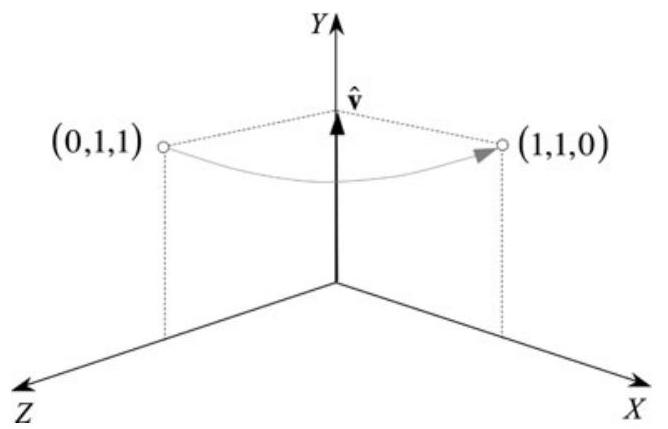
\includegraphics[max width=0.5\textwidth]{2023_01_16_a848224efad29cd66460g-121}
    \caption[short]{ti点$P(0,1,1)$围绕$y$轴旋转$90^{\circ}$到$P^{\prime}(1,1,0)$tle}
\end{figure}

现在我们可以写出
$$
\begin{aligned}
q p q^{-1} & =\mathbf{R}\left(q^{-1}\right) \mathbf{L}(q) p \\
& =\left[\begin{array}{cccc}
s & x & y & z \\
-x & s & -z & y \\
-y & z & s & -x \\
-z & -y & x & s
\end{array}\right]\left[\begin{array}{cccc}
s & -x & -y & -z \\
x & s & -z & y \\
y & z & s & -x \\
z & -y & x & s
\end{array}\right]\left[\begin{array}{c}
0 \\
x_{p} \\
y_{p} \\
z_{p}
\end{array}\right] \\
& =\left[\begin{array}{cccc}
1 & 0 & 0 & 0 \\
0 & 1-2\left(y^{2}+z^{2}\right) & 2(x y-s z) & 2(x z+s y) \\
0 & 2(x y+s z) & 1-2\left(x^{2}+z^{2}\right) & 2(y z-s x) \\
0 & 2(x z-s y) & 2(y z+s x) & 1-2\left(x^{2}+y^{2}\right)
\end{array}\right]\left[\begin{array}{c}
0 \\
x_{p} \\
y_{p} \\
z_{p}
\end{array}\right] .
\end{aligned}
$$
如果忽略第一行和第一列,矩阵将计算$\mathbf{p}^{\prime}$:
$$
\mathbf{p}^{\prime}=\left[\begin{array}{ccc}
1-2\left(y^{2}+z^{2}\right) & 2(x y-s z) & 2(x z+s y) \\
2(x y+s z) & 1-2\left(x^{2}+z^{2}\right) & 2(y z-s x) \\
2(x z-s y) & 2(y z+s x) & 1-2\left(x^{2}+y^{2}\right)
\end{array}\right]\left[\begin{array}{l}
x_{p} \\
y_{p} \\
z_{p}
\end{array}\right]
$$
这和(7.16)是一样的!

\subsection{几何验证}
让我们通过围绕$y$轴旋转点$(0,1,1), 90^{\circ}$来说明(7.15)的作用,如图7.7所示。四元数采用这种形式
$$
q=\left[\cos \frac{1}{2} \theta, \sin \frac{1}{2} \theta \hat{\mathbf{v}}\right]
$$
这意味着$\theta=90^{\circ}$和$\hat{\mathbf{v}}=\mathbf{j}$,因此,
$$
q=\left[\cos 45^{\circ}, \sin 45^{\circ} \hat{\mathbf{j}}\right]
$$
因此
$$
s=\frac{\sqrt{2}}{2}, \quad x=0, \quad y=\frac{\sqrt{2}}{2}, \quad z=0 .
$$
在(7.15)中代入这些值给出
$$
\begin{aligned}
\mathbf{p}^{\prime} & =\left[\begin{array}{ccc}
2\left(s^{2}+x^{2}\right)-1 & 2(x y-s z) & 2(x z+s y) \\
2(x y+s z) & 2\left(s^{2}+y^{2}\right)-1 & 2(y z-s x) \\
2(x z-s y) & 2(y z+s x) & 2\left(s^{2}+z^{2}\right)-1
\end{array}\right]\left[\begin{array}{l}
x_{p} \\
y_{p} \\
z_{p}
\end{array}\right] \\
{\left[\begin{array}{l}
1 \\
1 \\
0
\end{array}\right] } & =\left[\begin{array}{ccc}
0 & 0 & 1 \\
0 & 1 & 0 \\
-1 & 0 & 0
\end{array}\right]\left[\begin{array}{l}
0 \\
1 \\
1
\end{array}\right]
\end{aligned}
$$
其中$(0,1,1)$被旋转为$(1,1,0)$,这是正确的。

现在我们有了一个变换,可以让一个点绕任意轴旋转,这个轴与原点相交而没有欧拉变换带来的万向节锁定问题。

在继续之前,让我们再看一个例子。让我们对一个向量$\mathbf{v}=\mathbf{i}+\mathbf{k}$通过原点执行$180^{\circ}$旋转。首先,我们会故意忘记把这个向量转换成单位向量,只是为了看看最终矩阵会发生什么。四元数采用这种形式
$$
q=\left[\cos \frac{1}{2} \theta, \sin \frac{1}{2} \theta \hat{\mathbf{v}}\right]
$$
但是我们将使用指定的$\mathbf{v}$。因此,当使用$\theta=180^{\circ}$
$$
s=0, \quad x=1, \quad y=0, \quad z=1 .
$$
在(7.15)中代入这些值给出
$$
\begin{aligned}
\mathbf{p}^{\prime} & =\left[\begin{array}{ccc}
2\left(s^{2}+x^{2}\right)-1 & 2(x y-s z) & 2(x z+s y) \\
2(x y+s z) & 2\left(s^{2}+y^{2}\right)-1 & 2(y z-s x) \\
2(x z-s y) & 2(y z+s x) & 2\left(s^{2}+z^{2}\right)-1
\end{array}\right]\left[\begin{array}{l}
x_{p} \\
y_{p} \\
z_{p}
\end{array}\right] \\
& =\left[\begin{array}{ccc}
1 & 0 & 2 \\
0 & -1 & 0 \\
2 & 0 & 1
\end{array}\right]\left[\begin{array}{l}
1 \\
0 \\
0
\end{array}\right]
\end{aligned}
$$
它看起来一点也不像旋转矩阵,这提醒我们用单位向量来表示轴是多么重要。让我们重复这些计算,将向量归一化为$\hat{\mathbf{v}}=\frac{1}{\sqrt{2}} \mathbf{i}+\frac{1}{\sqrt{2}} \mathbf{k}$:
$$
s=0, \quad x=\frac{1}{\sqrt{2}}, \quad y=0, \quad z=\frac{1}{\sqrt{2}} .
$$
在(7.15)中代入这些值给出
$$
\begin{aligned}
\mathbf{p}^{\prime} & =\left[\begin{array}{ccc}
2\left(s^{2}+x^{2}\right)-1 & 2(x y-s z) & 2(x z+s y) \\
2(x y+s z) & 2\left(s^{2}+y^{2}\right)-1 & 2(y z-s x) \\
2(x z-s y) & 2(y z+s x) & 2\left(s^{2}+z^{2}\right)-1
\end{array}\right]\left[\begin{array}{l}
x_{p} \\
y_{p} \\
z_{p}
\end{array}\right] \\
{\left[\begin{array}{l}
0 \\
0 \\
1
\end{array}\right] } & =\left[\begin{array}{ccc}
0 & 0 & 1 \\
0 & -1 & 0 \\
1 & 0 & 0
\end{array}\right]\left[\begin{array}{l}
1 \\
0 \\
0
\end{array}\right]
\end{aligned}
$$
它不仅看起来像一个旋转矩阵,而且行列式为1,并将点$(1,0,0)$旋转到$(0,0,1)$,如图7.8所示。

\begin{figure}[h!]
    \centering
    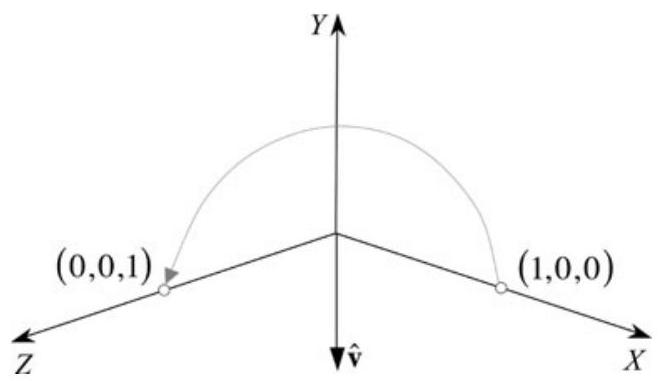
\includegraphics[max width=0.5\textwidth]{2023_01_16_a848224efad29cd66460g-123}
    \caption[short]{点$(1,0,0)$围绕向量$\hat{\mathbf{v}}$旋转$180^{\circ}$到$(0,0,1)$}
\end{figure}

\section{多个旋转}
假设一个向量或参考系受到$q_{1}$和$q_{2}$指定的两次旋转。有一种诱惑是将两个四元数转换为各自的矩阵并将矩阵相乘。然而,这并不是结合旋转的最有效的方法。最好将旋转累积为四元数,然后在需要时转换为矩阵符号。

为了说明这一点,考虑纯四元数$p$受到第一个四元数$q_{1}$的影响:
$$
q_{1} p q_{1}^{-1}
$$
后面跟着第二个四元数$q_{2}$
$$
q_{2}\left(q_{1} p q_{1}^{-1}\right) q_{2}^{-1}
$$
这可以表示为
$$
\left(q_{2} q_{1}\right) p\left(q_{2} q_{1}\right)^{-1} .
$$
可以相应地添加额外的四元数。让我们用两个例子来说明这一点。

为了简单起见,第一个四元数$q_{1}$围绕$y$-轴旋转$30^{\circ}$:
$$
q_{1}=\left[\cos 15^{\circ}, \sin 15^{\circ} \mathbf{j}\right] .
$$
第二个四元数$q_{2}$也围绕$y$轴旋转$60^{\circ}$:
$$
q_{2}=\left[\cos 30^{\circ}, \sin 30^{\circ} \mathbf{j}\right] .
$$
两个四元数一起围绕$y$轴旋转$90^{\circ}$。为了累积这些旋转,我们将它们相乘:
$$
\begin{aligned}
q_{1} q_{2} & =\left[\cos 15^{\circ}, \sin 15^{\circ} \mathbf{j}\right]\left[\cos 30^{\circ}, \sin 30^{\circ} \mathbf{j}\right] \\
& =\left[\cos 15^{\circ} \cos 30^{\circ}-\sin 15^{\circ} \sin 30^{\circ}, \cos 15^{\circ} \sin 30^{\circ} \mathbf{j}+\cos 30^{\circ} \sin 15^{\circ} \mathbf{j}\right] \\
& =\left[\frac{\sqrt{2}}{2}, \frac{\sqrt{2}}{2} \mathbf{j}\right]
\end{aligned}
$$
它是一个四元数,围绕y轴旋转。使用矩阵(7.15)我们有
$$
\begin{aligned}
\mathbf{p}^{\prime} & =\left[\begin{array}{ccc}
2\left(s^{2}+x^{2}\right)-1 & 2(x y-s z) & 2(x z+s y) \\
2(x y+s z) & 2\left(s^{2}+y^{2}\right)-1 & 2(y z-s x) \\
2(x z-s y) & 2(y z+s x) & 2\left(s^{2}+z^{2}\right)-1
\end{array}\right]\left[\begin{array}{l}
x_{p} \\
y_{p} \\
z_{p}
\end{array}\right] \\
& =\left[\begin{array}{ccc}
0 & 0 & 1 \\
0 & 1 & 0 \\
-1 & 0 & 0
\end{array}\right]\left[\begin{array}{c}
x_{p} \\
y_{p} \\
z_{p}
\end{array}\right]
\end{aligned}
$$
它围绕y轴旋转$90^{\circ}$。

第二个例子,让我们求四元数的值。第一个四元数$q_{1}$围绕$x$-轴旋转$90^{\circ}$, $q_{2}$围绕$y$-轴旋转$90^{\circ}$:

$$
\begin{aligned}
q_{1} & =\left[\frac{\sqrt{2}}{2}, \frac{\sqrt{2}}{2} \mathbf{i}\right] \\
q_{2} & =\left[\frac{\sqrt{2}}{2}, \frac{\sqrt{2}}{2} \mathbf{j}\right] \\
p & =[0, \mathbf{i}+\mathbf{j}]
\end{aligned}
$$
因此,
$$
\begin{aligned}
q_{2} q_{1} & =\left[\frac{\sqrt{2}}{2}, \frac{\sqrt{2}}{2} \mathbf{j}\right]\left[\frac{\sqrt{2}}{2}, \frac{\sqrt{2}}{2} \mathbf{i}\right] \\
& =\left[\frac{1}{2}, \frac{\sqrt{2}}{2} \frac{\sqrt{2}}{2} \mathbf{i}+\frac{\sqrt{2}}{2} \frac{\sqrt{2}}{2} \mathbf{j}-\frac{1}{2} \mathbf{k}\right] \\
& =\left[\frac{1}{2}, \frac{1}{2} \mathbf{i}+\frac{1}{2} \mathbf{j}-\frac{1}{2} \mathbf{k}\right] \\
\left(q_{2} q_{1}\right)^{-1} & =\left[\frac{1}{2},-\frac{1}{2} \mathbf{i}-\frac{1}{2} \mathbf{j}+\frac{1}{2} \mathbf{k}\right] \\
\left(q_{2} q_{1}\right) p & =\left[\frac{1}{2}, \frac{1}{2} \mathbf{i}+\frac{1}{2} \mathbf{j}-\frac{1}{2} \mathbf{k}\right][0, \mathbf{i}+\mathbf{j}] \\
& =\left[-\frac{1}{2}-\frac{1}{2}, \frac{1}{2}(\mathbf{i}+\mathbf{j})+\frac{1}{2} \mathbf{i}-\frac{1}{2} \mathbf{j}\right] \\
& =[-1, \mathbf{i}] \\
\left(q_{2} q_{1}\right) p\left(q_{2} q_{1}\right)^{-1} & =[-1, \mathbf{i}]\left[\frac{1}{2},-\frac{1}{2} \mathbf{i}-\frac{1}{2} \mathbf{j}+\frac{1}{2} \mathbf{k}\right] \\
& =\left[-\frac{1}{2}+\frac{1}{2}, \frac{1}{2} \mathbf{i}+\frac{1}{2} \mathbf{j}-\frac{1}{2} \mathbf{k}+\frac{1}{2} \mathbf{i}-\frac{1}{2} \mathbf{j}-\frac{1}{2} \mathbf{k}\right] \\
& =[0, \mathbf{i}-\mathbf{k}] .
\end{aligned}
$$
因此,点$(1,1,0)$被旋转到$(1,0,-1)$,这是正确的。

\section{特征值和特征向量}
虽然(7.15)无疑是一个旋转矩阵,但我们可以通过计算它的特征值和特征向量来获得进一步的证据。特征值应该是$\theta$,其中
$$
\operatorname{Tr}\left(q p q^{-1}\right)=1+2 \cos \theta
$$
$\operatorname{Tr}$是迹(trace)函数,它是矩阵中对角线元素的和。

$(7.15)$的迹是
$$
\begin{aligned}
\operatorname{Tr}\left(q p q^{-1}\right) & =2\left(s^{2}+x^{2}\right)-1+2\left(s^{2}+y^{2}\right)-1+2\left(s^{2}+z^{2}\right)-1 \\
& =4 s^{2}+2\left(s^{2}+x^{2}+y^{2}+z^{2}\right)-3 \\
& =4 s^{2}-1 \\
& =4 \cos ^{2} \frac{1}{2} \theta-1 \\
& =4 \cos \theta+4 \sin ^{2} \frac{1}{2} \theta-1 \\
& =4 \cos \theta+2-2 \cos \theta-1 \\
& =1+2 \cos \theta
\end{aligned}
$$
且
$$
\cos \theta=\frac{1}{2}\left(\operatorname{Tr}\left(q p q^{-1}\right)-1\right) .
$$
为了计算(7.15)的特征向量,我们使用附录中导出的三个方程:
$$
\begin{aligned}
& x_{v}=\left(a_{22}-1\right)\left(a_{33}-1\right)-a_{23} a_{32} \\
& y_{v}=\left(a_{33}-1\right)\left(a_{11}-1\right)-a_{31} a_{13} \\
& z_{v}=\left(a_{11}-1\right)\left(a_{22}-1\right)-a_{12} a_{21} .
\end{aligned}
$$
因此,
$$
\begin{aligned}
x_{v} & =\left(2\left(s^{2}+y^{2}\right)-2\right)\left(2\left(s^{2}+z^{2}\right)-2\right)-2(y z-s x) 2(y z+s x) \\
& =4\left(s^{2}+y^{2}-1\right)\left(s^{2}+z^{2}-1\right)-4\left(y^{2} z^{2}-s^{2} x^{2}\right) \\
& =4\left(\left(x^{2}+z^{2}\right)\left(x^{2}+y^{2}\right)-y^{2} z^{2}+s^{2} x^{2}\right) \\
& =4\left(x^{4}+x^{2} y^{2}+x^{2} z^{2}+z^{2} y^{2}-y^{2} z^{2}+s^{2} x^{2}\right) \\
& =4 x^{2}\left(s^{2}+x^{2}+y^{2}+z^{2}\right) \\
& =4 x^{2} .
\end{aligned}
$$
类似地,$y_{v}= 4y ^{2}$和$z_{v}= 4z ^{2}$,它们确认特征向量具有与四元数向量相关的分量。平方项应该不奇怪,因为三元$q p q^{-1}$包括三个四元数的乘积。让我们用与图7.8相关的矩阵来测试这些公式,它围绕向量$\hat{\mathbf{v}}=\frac{1}{\sqrt{2}} \mathbf{i}+\frac{1}{\sqrt{2}} \mathbf{k}$旋转一个点$180^{\circ}$:
$$
\mathbf{M}=\left[\begin{array}{lll}
a_{11} & a_{12} & a_{13} \\
a_{21} & a_{22} & a_{23} \\
a_{31} & a_{32} & a_{33}
\end{array}\right]=\left[\begin{array}{ccc}
0 & 0 & 1 \\
0 & -1 & 0 \\
1 & 0 & 0
\end{array}\right]
$$
因此,
$$
\begin{aligned}
& x_{v}=-2 \times-1-0=2 \\
& y_{v}=-1 \times-1-1 \times 1=0 \\
& z_{v}=-1 \times-2-0=2
\end{aligned}
$$
这证实了特征向量是$2 \mathbf{i}+2 \mathbf{k}$。

接下来,$\operatorname{Tr}(\mathbf{M})=-1$,因此
$$
\begin{aligned}
\cos \theta & =\frac{1}{2}\left(\operatorname{Tr}\left(q p q^{-1}\right)-1\right) \\
& =\frac{1}{2}((-1)-1) \\
& =-1 \\
\theta & =\pm 180^{\circ}
\end{aligned}
$$
这与之前的结果一致。

\section{绕偏移轴旋转}
现在我们有了一个表示四元数转子的矩阵,我们可以使用它来解决一些问题,例如使用与常规旋转变换相关的相同技术围绕偏轴旋转一个点。例如,在第六章中,我们使用了下面的符号
$$
\left[\begin{array}{c}
x^{\prime} \\
y^{\prime} \\
z^{\prime} \\
1
\end{array}\right]=\mathbf{T}_{t_{x}, 0, t_{z}} \mathbf{R}_{\beta, y} \mathbf{T}_{-t_{x}, 0,-t_{z}}\left[\begin{array}{c}
x \\
y \\
z \\
1
\end{array}\right]
$$
来绕与$y$-轴平行的固定轴旋转一点。因此,通过将矩阵$q p q^{-1}$替换为$\mathbf{R}_{\beta, y}$,我们有
$$
\left[\begin{array}{c}
x^{\prime} \\
y^{\prime} \\
z^{\prime} \\
1
\end{array}\right]=\mathbf{T}_{t_{x}, 0, t_{z}}\left(q p q^{-1}\right) \mathbf{T}_{-t_{x}, 0,-t_{z}}\left[\begin{array}{c}
x \\
y \\
z \\
1
\end{array}\right] .
$$
让我们通过旋转我们的单位立方体$90^{\circ}$来测试这一点,围绕与顶点4和6相交的垂直轴,如图7.9所示。

\begin{figure}[h!]
    \centering
    \subfigure[]{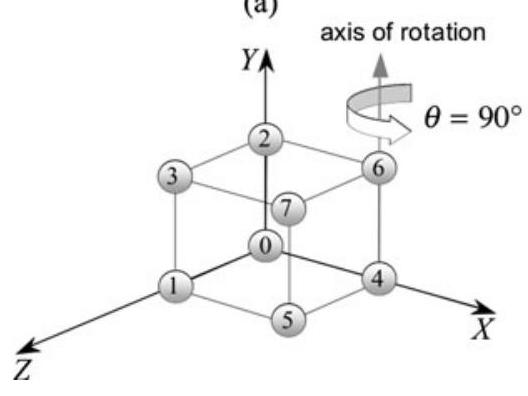
\includegraphics[max width=0.45\textwidth]{2023_01_16_a848224efad29cd66460g-127}}
    \subfigure[]{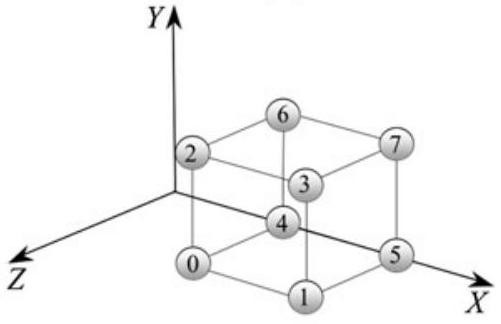
\includegraphics[max width=0.45\textwidth]{2023_01_16_a848224efad29cd66460g-127(1)}}
    \caption[short]{立方体围绕与顶点4和6相交的轴旋转$90^{\circ}$}
\end{figure}

实现这一点的单位范数四元数是
$$
q=\left[\cos 45^{\circ}, \sin 45^{\circ} \mathbf{j}\right]
$$
用纯四元数
$$
p=[0, \mathbf{p}]
$$
因此,
$$
s=\frac{\sqrt{2}}{2}, \quad x=0, \quad y=\frac{\sqrt{2}}{2}, \quad z=0
$$
用(7.15)的齐次形式
$$
\begin{aligned}
\mathbf{p}^{\prime} & =\left[\begin{array}{cccc}
2\left(s^{2}+x^{2}\right)-1 & 2(x y-s z) & 2(x z+s y) & 0 \\
2(x y+s z) & 2\left(s^{2}+y^{2}\right)-1 & 2(y z-s x) & 0 \\
2(x z-s y) & 2(y z+s x) & 2\left(s^{2}+z^{2}\right)-1 & 0 \\
0 & 0 & 1
\end{array}\right]\left[\begin{array}{c}
x_{p} \\
y_{p} \\
z_{p} \\
1
\end{array}\right] \\
& =\left[\begin{array}{cccc}
0 & 0 & 1 & 0 \\
0 & 1 & 0 & 0 \\
-1 & 0 & 0 & 0 \\
0 & 0 & 0 & 1
\end{array}\right]\left[\begin{array}{c}
x_{p} \\
y_{p} \\
z_{p} \\
1
\end{array}\right]
\end{aligned}
$$
另外两个矩阵是
$$
\begin{aligned}
\mathbf{T}_{-t_{x}, 0,0} & =\left[\begin{array}{cccc}
1 & 0 & 0 & -1 \\
0 & 1 & 0 & 0 \\
0 & 0 & 1 & 0 \\
0 & 0 & 0 & 1
\end{array}\right] \\
\mathbf{T}_{t_{x}, 0,0} & =\left[\begin{array}{llll}
1 & 0 & 0 & 1 \\
0 & 1 & 0 & 0 \\
0 & 0 & 1 & 0 \\
0 & 0 & 0 & 1
\end{array}\right] .
\end{aligned}
$$
将这三个矩阵相乘会得到
\begin{align}
\left[\begin{array}{cccc}
0 & 0 & 1 & 1 \\
0 & 1 & 0 & 0 \\
-1 & 0 & 0 & 1 \\
0 & 0 & 0 & 1
\end{array}\right]
\end{align}
虽然在数学上不正确,但下面的语句显示了矩阵(7.19)和表示单位立方体的坐标数组,后面是旋转后的立方体的坐标。
$$
\begin{gathered}
{\left[\begin{array}{cccc}
0 & 0 & 1 & 1 \\
0 & 1 & 0 & 0 \\
-1 & 0 & 0 & 1 \\
0 & 0 & 0 & 1
\end{array}\right]\left[\begin{array}{llllllll}
0 & 0 & 0 & 0 & 1 & 1 & 1 & 1 \\
0 & 0 & 1 & 1 & 0 & 0 & 1 & 1 \\
0 & 1 & 0 & 1 & 0 & 1 & 0 & 1 \\
1 & 1 & 1 & 1 & 1 & 1 & 1 & 1
\end{array}\right]} \\
=\left[\begin{array}{llllllll}
1 & 2 & 1 & 2 & 1 & 2 & 1 & 2 \\
0 & 0 & 1 & 1 & 0 & 0 & 1 & 1 \\
1 & 1 & 1 & 1 & 0 & 0 & 0 & 0 \\
1 & 1 & 1 & 1 & 1 & 1 & 1 & 1
\end{array}\right]
\end{gathered}
$$
这些坐标由图7.9确认。

\section{参考系}
乘积$q p q^{-1}$用于旋转与四元数$q$相关的向量的点,而三元$q^{-1} p q$可用于旋转与同一向量相关的相反方向的点。但这种反向旋转也相当于改变了参照系。为了证明这一点,考虑绕$\mathbf{i}+\mathbf{k}$旋转参考系$180^{\circ}$的问题,如图7.10所示。这种旋转的单位范四元数是
$$
\begin{aligned}
q & =\left[\cos 90^{\circ}, \sin 90^{\circ}\left(\frac{1}{\sqrt{2}} \mathbf{i}+\frac{1}{\sqrt{2}} \mathbf{k}\right)\right] \\
& =\left[0, \frac{\sqrt{2}}{2} \mathbf{i}+\frac{\sqrt{2}}{2} \mathbf{k}\right] .
\end{aligned}
$$
因此
$$
s=0, \quad x=\frac{\sqrt{2}}{2}, \quad y=0, \quad z=\frac{\sqrt{2}}{2} .
$$
将这些值代入(7.17)得到
$$
\begin{aligned}
q^{-1} p q & =\left[\begin{array}{ccc}
2\left(s^{2}+x^{2}\right)-1 & 2(x y+s z) & 2(x z-s y) \\
2(x y-s z) & 2\left(s^{2}+y^{2}\right)-1 & 2(y z+s x) \\
2(x z+s y) & 2(y z-s x) & 2\left(s^{2}+z^{2}\right)-1
\end{array}\right]\left[\begin{array}{l}
x_{p} \\
y_{p} \\
z_{p}
\end{array}\right] \\
& =\left[\begin{array}{ccc}
0 & 0 & 1 \\
0 & -1 & 0 \\
1 & 0 & 0
\end{array}\right]\left[\begin{array}{l}
x_{p} \\
y_{p} \\
z_{p}
\end{array}\right]
\end{aligned}
$$
如果用它来处理单位立方体的坐标,会产生什么
$$
\begin{gathered}
{\left[\begin{array}{ccc}
0 & 0 & 1 \\
0 & -1 & 0 \\
1 & 0 & 0
\end{array}\right]\left[\begin{array}{cccccccc}
0 & 0 & 0 & 0 & 1 & 1 & 1 & 1 \\
0 & 0 & 1 & 1 & 0 & 0 & 1 & 1 \\
0 & 1 & 0 & 1 & 0 & 1 & 0 & 1
\end{array}\right]} \\
=\left[\begin{array}{cccccccc}
0 & 1 & 0 & 1 & 0 & 1 & 0 & 1 \\
0 & 0 & -1 & -1 & 0 & 0 & -1 & -1 \\
0 & 0 & 0 & 0 & 1 & 1 & 1 & 1
\end{array}\right] .
\end{gathered}
$$
此场景如图$7.10$所示。
\begin{figure}[h!]
    \centering
    \subfigure[]{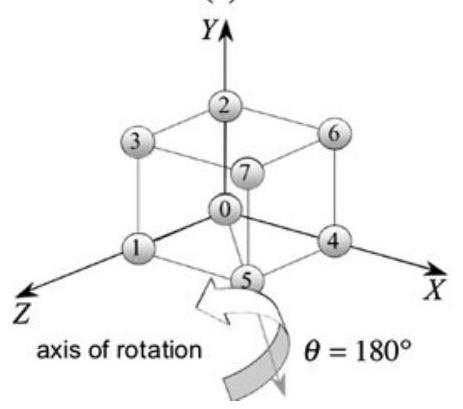
\includegraphics[max width=0.4\textwidth]{2023_01_16_a848224efad29cd66460g-129}}
    \subfigure[]{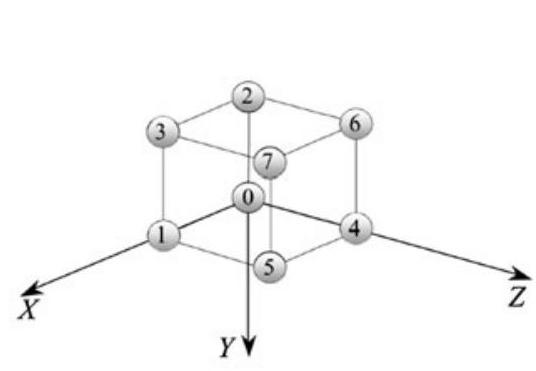
\includegraphics[max width=0.45\textwidth]{2023_01_16_a848224efad29cd66460g-129(1)}}
    \caption[short]{帧围绕向量$\mathbf{i}+\mathbf{k}$旋转$180^{\circ}$}
\end{figure}

\section{四元数插值}
像向量一样,四元数可以被插值以计算中间的四元数。然而,两个插值向量会产生第三个很容易可视化的向量,而两个插值四元数会产生第三个四元数,它充当转子,不能立即可视化。

向量的球面插值是
$$
\mathbf{v}=\frac{\sin (1-t) \theta}{\sin \theta} \mathbf{v}_{1}+\frac{\sin t \theta}{\sin \theta} \mathbf{v}_{2}
$$
其中$\theta$是向量之间的夹角,对于四元数不需要修改:
\begin{align}
q=\frac{\sin (1-t) \theta}{\sin \theta} q_{1}+\frac{\sin t \theta}{\sin \theta} q_{2}
\end{align}
因此,给出
$$
\begin{aligned}
& q_{1}=\left[s_{1}, x_{1} \mathbf{i}+y_{1} \mathbf{j}+z_{1} \mathbf{k}\right] \\
& q_{2}=\left[s_{2}, x_{2} \mathbf{i}+y_{2} \mathbf{j}+z_{2} \mathbf{k}\right]
\end{aligned}
$$
$\theta$由$q_{1}$和$q_{2}$的4D点积得到:
$$
\begin{aligned}
\cos \theta & =\frac{q_{1} \cdot q_{2}}{\left|q_{1}\right|\left|q_{2}\right|} \\
& =\frac{s_{1} s_{2}+x_{1} x_{2}+y_{1} y_{2}+z_{1} z_{2}}{\left|q_{1}\right|\left|q_{2}\right|}
\end{aligned}
$$
如果我们用的是单位范数四元数,那么
\begin{align}
    \cos \theta=s_{1} s_{2}+x_{1} x_{2}+y_{1} y_{2}+z_{1} z_{2} .
\end{align}
让我们在具有两个简单单位范数四元数的场景中使用(7.20)。

\begin{figure}[h!]
    \centering
    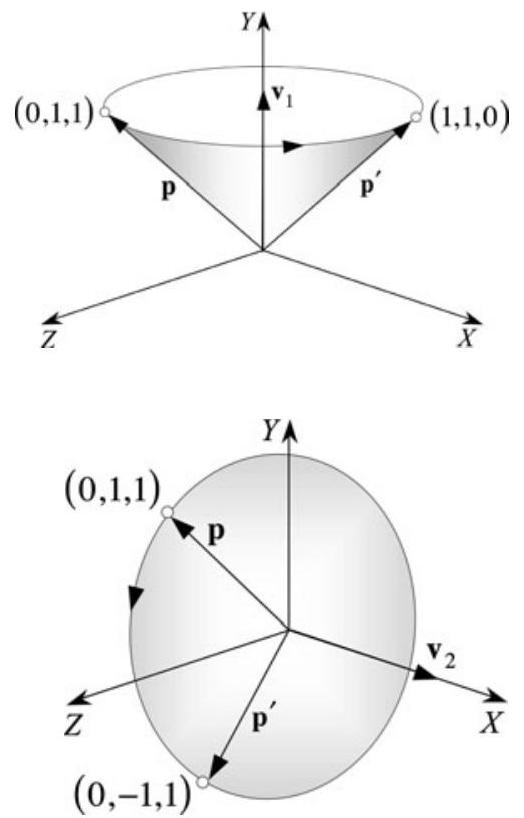
\includegraphics[max width=0.5\textwidth]{2023_01_16_a848224efad29cd66460g-130}
    \caption[short]{点$(0,1,1)$围绕向量$\mathbf{v}_{1}$旋转$90^{\circ}$到$(1,1,0)$}
\end{figure}

\begin{figure}[h!]
    \centering
    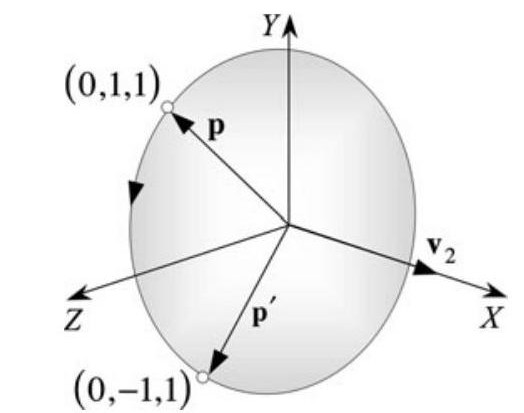
\includegraphics[max width=0.5\textwidth]{2023_01_16_a848224efad29cd66460g-130(1)}
    \caption[short]{点$(0,1,1)$围绕向量$\mathbf{v}_{2}$旋转$90^{\circ}$到$(0,-1,1)$}
\end{figure}

图$7.11$显示了一个这样的场景,其中点$(0,1,1)$绕 $q_{1}$的轴$\mathbf{v}_{1}$旋转$90^{\circ}$。图$7.12$显示了另一种场景,其中相同的点$(0,1,1)$绕 $q_{2}$的轴$\mathbf{v}_{2}$旋转$90^{\circ}$。四元数是

$$
\begin{aligned}
& q_{1}=\left[\cos 45^{\circ}, \sin 45^{\circ} \mathbf{j}\right]=\left[\frac{\sqrt{2}}{2}, \frac{\sqrt{2}}{2} \mathbf{j}\right] \\
& q_{2}=\left[\cos 45^{\circ}, \sin 45^{\circ} \mathbf{i}\right]=\left[\frac{\sqrt{2}}{2}, \frac{\sqrt{2}}{2} \mathbf{i}\right] .
\end{aligned}
$$
因此,使用(7.21)
$$
\begin{aligned}
\cos \theta & =\frac{\sqrt{2}}{2} \frac{\sqrt{2}}{2}=0.5 \\
\theta & =60^{\circ} .
\end{aligned}
$$
在继续之前,让我们计算两个四元数乘积的矩阵。对于$q_{1}$:
$$
s=\frac{\sqrt{2}}{2}, \quad x=0, \quad y=\frac{\sqrt{2}}{2}, \quad z=0
$$
当代入(7.15)得到
\begin{align}
\begin{aligned}
\mathbf{p}_{1}^{\prime} & =\left[\begin{array}{ccc}
2\left(s^{2}+x^{2}\right)-1 & 2(x y-s z) & 2(x z+s y) \\
2(x y+s z) & 2\left(s^{2}+y^{2}\right)-1 & 2(y z-s x) \\
2(x z-s y) & 2(y z+s x) & 2\left(s^{2}+z^{2}\right)-1
\end{array}\right]\left[\begin{array}{l}
x_{p} \\
y_{p} \\
z_{p}
\end{array}\right] \\
& =\left[\begin{array}{ccc}
0 & 0 & 1 \\
0 & 1 & 0 \\
-1 & 0 & 0
\end{array}\right]\left[\begin{array}{l}
x_{p} \\
y_{p} \\
z_{p}
\end{array}\right] .
\end{aligned}
\end{align}
将坐标$(0,1,1)$代入$(7.22)$
$$
\left[\begin{array}{l}
1 \\
1 \\
0
\end{array}\right]=\left[\begin{array}{ccc}
0 & 0 & 1 \\
0 & 1 & 0 \\
-1 & 0 & 0
\end{array}\right]\left[\begin{array}{l}
0 \\
1 \\
1
\end{array}\right]
$$
这是正确的。

对于 $q_{2}$ :
$$
s=\frac{\sqrt{2}}{2}, \quad x=\frac{\sqrt{2}}{2}, \quad y=0, \quad z=0
$$
当代入$(7.15)$时,会得到
\begin{align}
\begin{aligned}
\mathbf{p}_{2}^{\prime} & =\left[\begin{array}{ccc}
2\left(s^{2}+x^{2}\right)-1 & 2(x y-s z) & 2(x z+s y) \\
2(x y+s z) & 2\left(s^{2}+y^{2}\right)-1 & 2(y z-s x) \\
2(x z-s y) & 2(y z+s x) & 2\left(s^{2}+z^{2}\right)-1
\end{array}\right]\left[\begin{array}{l}
x_{p} \\
y_{p} \\
z_{p}
\end{array}\right] \\
& =\left[\begin{array}{ccc}
1 & 0 & 0 \\
0 & 0 & -1 \\
0 & 1 & 0
\end{array}\right]\left[\begin{array}{c}
x_{p} \\
y_{p} \\
z_{p}
\end{array}\right] .
\end{aligned}
\end{align}
将坐标$(0,1,1)$代入$(7.23)$
$$
\left[\begin{array}{c}
0 \\
-1 \\
1
\end{array}\right]=\left[\begin{array}{ccc}
1 & 0 & 0 \\
0 & 0 & -1 \\
0 & 1 & 0
\end{array}\right]\left[\begin{array}{l}
0 \\
1 \\
1
\end{array}\right]
$$
这是正确的。

\begin{figure}[h!]
    \centering
    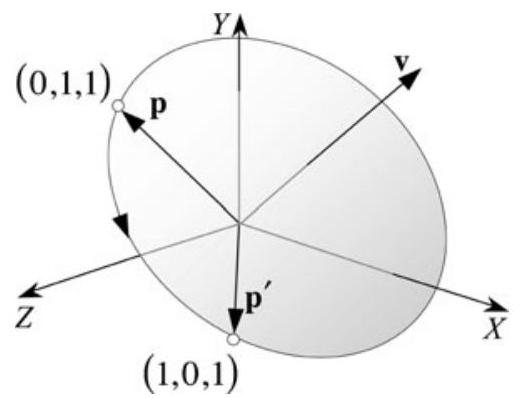
\includegraphics[max width=0.5\textwidth]{2023_01_16_a848224efad29cd66460g-132}
    \caption[short]{点$(0,1,1)$围绕向量$\mathbf{v}$旋转$90^{\circ}$到$(1,0,1)$}
\end{figure}

使用(7.20)和$t=0.5$计算插值四元数的中间位置,其向量在$x$ -和$y$-轴之间的$45^{\circ}$,如图7.13所示。我们已经知道$\theta=60^{\circ}$,因此$\sin \theta=\sqrt{3}/ 2$:
$$
\begin{aligned}
q & =\frac{\sin (1-t) \theta}{\sin \theta} q_{1}+\frac{\sin t \theta}{\sin \theta} q_{2} \\
& =\frac{\sin \frac{1}{2} 60^{\circ}}{\sin 60^{\circ}}\left[\frac{\sqrt{2}}{2}, \frac{\sqrt{2}}{2} \mathbf{j}\right]+\frac{\sin \frac{1}{2} 60^{\circ}}{\sin 60^{\circ}}\left[\frac{\sqrt{2}}{2}, \frac{\sqrt{2}}{2} \mathbf{i}\right]\\
& =\frac{1}{\sqrt{3}}\left[\frac{\sqrt{2}}{2}, \frac{\sqrt{2}}{2} \mathbf{j}\right]+\frac{1}{\sqrt{3}}\left[\frac{\sqrt{2}}{2}, \frac{\sqrt{2}}{2} \mathbf{i}\right] \\
& =\left[\frac{\sqrt{2}}{\sqrt{3}}, \frac{1}{\sqrt{6}} \mathbf{i}+\frac{1}{\sqrt{6}} \mathbf{j}\right]
\end{aligned}
$$
其中
$$
s=\frac{\sqrt{2}}{\sqrt{3}}, \quad x=\frac{1}{\sqrt{6}}, \quad y=\frac{1}{\sqrt{6}}, \quad z=0
$$
当代入$(7.15)$时,会得到
\begin{align}
    \begin{aligned}
\mathbf{p}^{\prime} & =\left[\begin{array}{ccc}
2\left(s^{2}+x^{2}\right)-1 & 2(x y-s z) & 2(x z+s y) \\
2(x y+s z) & 2\left(s^{2}+y^{2}\right)-1 & 2(y z-s x) \\
2(x z-s y) & 2(y z+s x) & 2\left(s^{2}+z^{2}\right)-1
\end{array}\right]\left[\begin{array}{l}
x_{p} \\
y_{p} \\
z_{p}
\end{array}\right] \\
& =\left[\begin{array}{ccc}
\frac{2}{3} & \frac{1}{3} & \frac{2}{3} \\
\frac{1}{3} & \frac{2}{3} & -\frac{2}{3} \\
-\frac{2}{3} & \frac{2}{3} & \frac{1}{3}
\end{array}\right]\left[\begin{array}{l}
x_{p} \\
y_{p} \\
z_{p}
\end{array}\right] .
\end{aligned}
\end{align}
将坐标$(0,1,1)$代入$(7.24)$
\begin{align}
    \left[\begin{array}{l}
        1 \\
        0 \\
        1
        \end{array}\right]=\left[\begin{array}{ccc}
        \frac{2}{3} & \frac{1}{3} & \frac{2}{3} \\
        \frac{1}{3} & \frac{2}{3} & -\frac{2}{3} \\
        -\frac{2}{3} & \frac{2}{3} & \frac{1}{3}
        \end{array}\right]\left[\begin{array}{l}
        0 \\
        1 \\
        1
        \end{array}\right]
\end{align}
这得到点$(1,0,1)$。

使用球面插补器的原因之一是它线性插补两个单位范数四元数之间的角度,这在它们之间创建了一个恒定的角速度。然而,可视化四元数的一个问题是,它们驻留在一个四维空间中,并创建了一个半径等于四元数范数的超球面。对于我们的3D大脑来说,这是很难想象的。然而,我们可以让自己相信,我们可以通过一个简单的草图来了解正在发生的事情,如图7.14所示,在那里我们看到了超球面的一部分和两个四元数$q_{1}$和$q_{2}$。在这个例子中,角度$\phi$是插值值$t$之间的常数角。球面插值器还确保插值四元数的范数保持不变,防止任何不必要的缩放。

\begin{figure}[h!]
    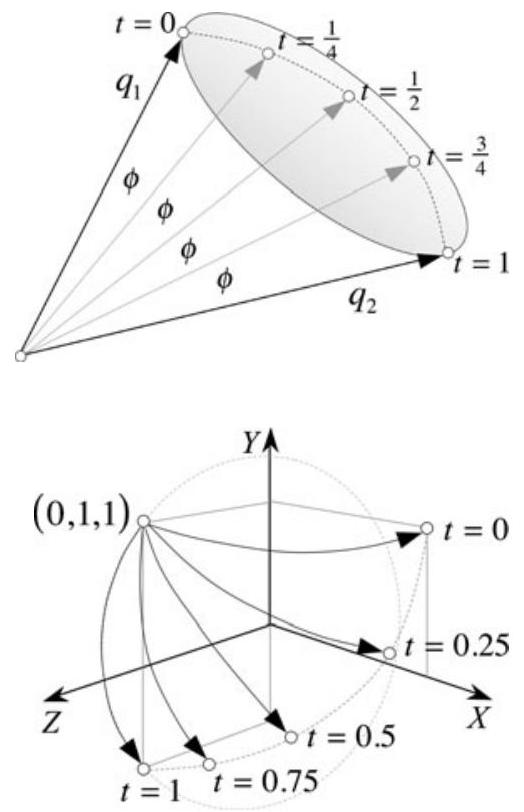
\includegraphics[max width=0.5\textwidth, center]{2023_01_16_a848224efad29cd66460g-133}
    \caption[short]{$q_{1}$和$q_{2}$之间的球面插值}
\end{figure}

\begin{figure}[h!]
    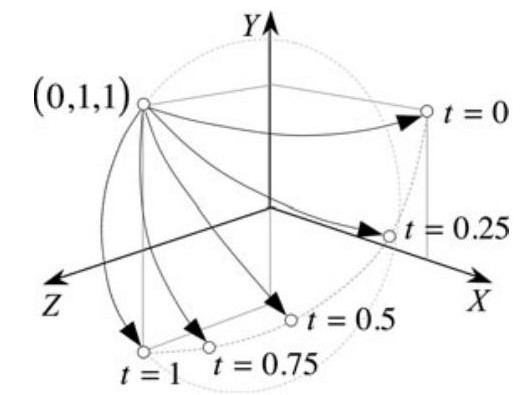
\includegraphics[max width=0.5\textwidth, center]{2023_01_16_a848224efad29cd66460g-133(1)}
    \caption[short]{显示插值四元数动作的草图}
\end{figure}

图$7.15$提供了另一个草图,以帮助可视化发生了什么。例如,当$t=0$时,插值的四元数是$q_{1}$,它将点$(0,1,1)$旋转到$(1,1,0)$;当$t=1$时,插值的四元数是$q_{2}$,它将点$(0,1,1)$旋转到$(0,1,1)$。当$t=0.5$时,插值四元数将点$(0,1,1)$旋转到如上计算的$(1,0,1)$。另外两条曲线显示了$t=0.25$和$t=0.75$时的情况。

插值的一个自然结果是,对于$t=0$和$t=1$,旋转角度为$90^{\circ}$,但是对于$t=0.5$,旋转角度(特征值)大约为$70.5^{\circ}$。对于$t$的其他值产生相应的角度。

\section{将旋转矩阵转换为四元数}
矩阵变换等价于$q p q^{-1}$为
$$
\begin{aligned}
q p q^{-1} & =\left[\begin{array}{ccc}
2\left(s^{2}+x^{2}\right)-1 & 2(x y-s z) & 2(x z+s y) \\
2(x y+s z) & 2\left(s^{2}+y^{2}\right)-1 & 2(y z-s x) \\
2(x z-s y) & 2(y z+s x) & 2\left(s^{2}+z^{2}\right)-1
\end{array}\right]\left[\begin{array}{l}
x_{p} \\
y_{p} \\
z_{p}
\end{array}\right] \\
& =\left[\begin{array}{lll}
a_{11} & a_{12} & a_{13} \\
a_{21} & a_{22} & a_{23} \\
a_{31} & a_{32} & a_{33}
\end{array}\right]\left[\begin{array}{l}
x_{p} \\
y_{p} \\
z_{p}
\end{array}\right] .
\end{aligned}
$$
对矩阵的检查表明,通过组合各种元素,我们可以分离出四元数$s, x, y, z$的项。例如,通过将项$a_{11}+a_{22}+a_{33}$相加,我们得到
$$
\begin{aligned}
a_{11}+a_{22}+a_{33} & =\left(2\left(s^{2}+x^{2}\right)-1\right)+\left(2\left(s^{2}+y^{2}\right)-1\right)+\left(2\left(s^{2}+z^{2}\right)-1\right) \\
& =6 s^{2}+2\left(x^{2}+y^{2}+z^{2}\right)-3 \\
& =4 s^{2}-1
\end{aligned}
$$
因此,
$$
s=\pm \frac{1}{2} \sqrt{1+a_{11}+a_{22}+a_{33}} .
$$
为了分离出$x, y$和$z$
$$
\begin{aligned}
& x=\frac{1}{4 s}\left(a_{32}-a_{23}\right) \\
& y=\frac{1}{4 s}\left(a_{13}-a_{31}\right) \\
& z=\frac{1}{4 s}\left(a_{21}-a_{12}\right) .
\end{aligned}
$$
我们可以用矩阵(7.25)确认它们的正确性:
$$
\begin{aligned}
& \left[\begin{array}{lll}a_{11} & a_{12} & a_{13} \\a_{21} & a_{22} & a_{23} \\a_{31} & a_{32} & a_{33}\end{array}\right]=\left[\begin{array}{ccc}\frac{2}{3} & \frac{1}{3} & \frac{2}{3} \\\frac{1}{3} & \frac{2}{3} & -\frac{2}{3} \\-\frac{2}{3} & \frac{2}{3} & \frac{1}{3}\end{array}\right] \\
& s=\pm \frac{1}{2} \sqrt{1+a_{11}+a_{22}+a_{33}}=\pm \frac{1}{2} \sqrt{1+\frac{2}{3}+\frac{2}{3}+\frac{1}{3}}=\frac{\sqrt{2}}{\sqrt{3}} \\
& x=\frac{1}{4 s}\left(a_{32}-a_{23}\right)=\frac{\sqrt{3}}{4 \sqrt{2}}\left(\frac{2}{3}+\frac{2}{3}\right)=\frac{1}{\sqrt{6}} \\
& y=\frac{1}{4 s}\left(a_{13}-a_{31}\right)=\frac{\sqrt{3}}{4 \sqrt{2}}\left(\frac{2}{3}+\frac{2}{3}\right)=\frac{1}{\sqrt{6}} \\
& z=\frac{1}{4 s}\left(a_{21}-a_{12}\right)=\frac{\sqrt{3}}{4 \sqrt{2}}\left(\frac{1}{3}-\frac{1}{3}\right)=0
\end{aligned}
$$
与原始值一致。

例如,$s$的值接近于零,这可能会使$x, y, z$的值不可靠。因此,其他组合是可用的:
$$
\begin{aligned}
x & =\pm \frac{1}{2} \sqrt{1+a_{11}-a_{22}-a_{33}} \\
y & =\frac{1}{4 x}\left(a_{12}+a_{21}\right) \\
z & =\frac{1}{4 x}\left(a_{13}+a_{31}\right)\\
s & =\frac{1}{4 x}\left(a_{32}-a_{23}\right) \\
y & =\pm \frac{1}{2} \sqrt{1-a_{11}+a_{22}-a_{33}} \\
x & =\frac{1}{4 y}\left(a_{12}+a_{21}\right) \\
z & =\frac{1}{4 y}\left(a_{23}+a_{32}\right) \\
s & =\frac{1}{4 y}\left(a_{13}-a_{31}\right) \\
z & =\pm \frac{1}{2} \sqrt{1-a_{11}-a_{22}+a_{33}} \\
x & =\frac{1}{4 z}\left(a_{13}+a_{31}\right) \\
y & =\frac{1}{4 z}\left(a_{23}+a_{32}\right) \\
s & =\frac{1}{4 z}\left(a_{21}-a_{12}\right) .
\end{aligned}
$$

% $$
% \begin{aligned}

% \end{aligned}
% $$

\section{欧拉角转换到四元数}
在第6章中,我们发现旋转变换$\mathbf{R}_{\alpha, x}, \mathbf{R}_{\beta, y}$和$\mathbf{R}_{\gamma, z}$可以组合起来创建12个三重组合来表示一个复合旋转。现在让我们看看这样的变换是如何用四元数表示的。

为了演示该技术,我们必须从12种组合中选择一种,然后可以使用相同的技术转换其他组合。例如,让我们选择序列$\mathbf{R}_{\gamma, z} \mathbf{R}_{\beta, y} \mathbf{R}_{\alpha, x}$,其中等价的四元数是
$$
\begin{aligned}
& q_{x}=\left[\cos \frac{1}{2} \alpha, \sin \frac{1}{2} \alpha \mathbf{i}\right] \\
& q_{y}=\left[\cos \frac{1}{2} \beta, \sin \frac{1}{2} \beta \mathbf{j}\right] \\
& q_{z}=\left[\cos \frac{1}{2} \gamma, \sin \frac{1}{2} \gamma \mathbf{k}\right]
\end{aligned}
$$
和
\begin{align}
    q=q_{z} q_{y} q_{x}
\end{align}
展开(7.26):
$$
\begin{aligned}
q=& \left[\cos \frac{1}{2} \gamma, \sin \frac{1}{2} \gamma \mathbf{k}\right]\left[\cos \frac{1}{2} \beta, \sin \frac{1}{2} \beta \mathbf{j}\right]\left[\cos \frac{1}{2} \alpha, \sin \frac{1}{2} \alpha \mathbf{i}\right] \\
=& \left[\cos \frac{1}{2} \gamma \cos \frac{1}{2} \beta,\right. \\
& \left.\cos \frac{1}{2} \gamma \sin \frac{1}{2} \beta \mathbf{j}+\cos \frac{1}{2} \beta \sin \frac{1}{2} \gamma \mathbf{k}-\sin \frac{1}{2} \gamma \sin \frac{1}{2} \beta \mathbf{i}\right]\left[\cos \frac{1}{2} \alpha, \sin \frac{1}{2} \alpha \mathbf{i}\right] \\
=& \left[\cos \frac{1}{2} \gamma \cos \frac{1}{2} \beta \cos \frac{1}{2} \alpha+\sin \frac{1}{2} \gamma \sin \frac{1}{2} \beta \sin \frac{1}{2} \alpha\right. \text {, } \\
& \cos \frac{1}{2} \gamma \cos \frac{1}{2} \beta \sin \frac{1}{2} \alpha \mathbf{i}+\cos \frac{1}{2} \alpha \cos \frac{1}{2} \gamma \sin \frac{1}{2} \beta \mathbf{j}+\cos \frac{1}{2} \alpha \cos \frac{1}{2} \beta \sin \frac{1}{2} \gamma \mathbf{k} \\
& \left.-\cos \frac{1}{2} \alpha \sin \frac{1}{2} \gamma \sin \frac{1}{2} \beta \mathbf{i}-\cos \frac{1}{2} \gamma \sin \frac{1}{2} \beta \sin \frac{1}{2} \alpha \mathbf{k}+\cos \frac{1}{2} \beta \sin \frac{1}{2} \gamma \sin \frac{1}{2} \alpha \mathbf{j}\right] \\
=& \left[\cos \frac{1}{2} \gamma \cos \frac{1}{2} \beta \cos \frac{1}{2} \alpha+\sin \frac{1}{2} \gamma \sin \frac{1}{2} \beta \sin \frac{1}{2} \alpha\right. \text {, } \\
& \left(\cos \frac{1}{2} \gamma \cos \frac{1}{2} \beta \sin \frac{1}{2} \alpha-\cos \frac{1}{2} \alpha \sin \frac{1}{2} \gamma \sin \frac{1}{2} \beta\right) \mathbf{i} \\
& \left(\cos \frac{1}{2} \alpha \cos \frac{1}{2} \gamma \sin \frac{1}{2} \beta+\cos \frac{1}{2} \beta \sin \frac{1}{2} \gamma \sin \frac{1}{2} \alpha\right) \mathbf{j} \\
& \left.\left(\cos \frac{1}{2} \alpha \cos \frac{1}{2} \beta \sin \frac{1}{2} \gamma-\cos \frac{1}{2} \gamma \sin \frac{1}{2} \beta \sin \frac{1}{2} \alpha\right) \mathbf{k}\right] \text {. }
\end{aligned}
$$
现在让我们以一致的顺序放置角度:
$$
\begin{aligned}
s & =\cos \frac{1}{2} \gamma \cos \frac{1}{2} \beta \cos \frac{1}{2} \alpha+\sin \frac{1}{2} \gamma \sin \frac{1}{2} \beta \sin \frac{1}{2} \alpha \\
x_{q} & =\cos \frac{1}{2} \gamma \cos \frac{1}{2} \beta \sin \frac{1}{2} \alpha-\sin \frac{1}{2} \gamma \sin \frac{1}{2} \beta \cos \frac{1}{2} \alpha \\
y_{q} & =\cos \frac{1}{2} \gamma \sin \frac{1}{2} \beta \cos \frac{1}{2} \alpha+\sin \frac{1}{2} \gamma \cos \frac{1}{2} \beta \sin \frac{1}{2} \alpha \\
z_{q} & =\sin \frac{1}{2} \gamma \cos \frac{1}{2} \beta \cos \frac{1}{2} \alpha-\cos \frac{1}{2} \gamma \sin \frac{1}{2} \beta \sin \frac{1}{2} \alpha
\end{aligned}
$$
其中
\begin{align}
    q=\left[s, x_{q} \mathbf{i}+y_{q} \mathbf{j}+z_{q} \mathbf{k}\right] .
\end{align}
让我们测试(7.27)。我们从三个旋转变换开始
$$
\begin{aligned}
\mathbf{R}_{\alpha, x} & =\left[\begin{array}{ccc}
1 & 0 & 0 \\
0 & \cos \alpha & -\sin \alpha \\
0 & \sin \alpha & \cos \alpha
\end{array}\right] \\
\mathbf{R}_{\beta, y} & =\left[\begin{array}{ccc}
\cos \beta & 0 & \sin \beta \\
0 & 1 & 0 \\
-\sin \beta & 0 & \cos \beta
\end{array}\right]\\
\mathbf{R}_{\gamma, z}& =\left[\begin{array}{ccc}
    \cos \gamma & -\sin \gamma & 0 \\
    \sin \gamma & \cos \gamma & 0 \\
    0 & 0 & 1
    \end{array}\right]
\end{aligned}
$$
然后
$$
\begin{aligned}
& \mathbf{R}_{\gamma, z} \mathbf{R}_{\beta, y} \mathbf{R}_{\alpha, x} \\
&= {\left[\begin{array}{ccc}
\cos \gamma \cos \beta & -\sin \gamma \cos \alpha+\cos \gamma \sin \beta \sin \alpha & \sin \gamma \sin \alpha+\cos \gamma \sin \beta \cos \alpha \\
\sin \gamma \cos \beta & \cos \gamma \cos \alpha+\sin \gamma \sin \beta \sin \alpha & -\cos \gamma \sin \alpha+\sin \gamma \sin \beta \cos \alpha \\
-\sin \beta & \cos \beta \sin \alpha & \cos \beta \cos \alpha
\end{array}\right] . }
\end{aligned}
$$
令$\alpha=\beta=\gamma=90^{\circ}$,那么
$$
\mathbf{R}_{90^{\circ}, z} \mathbf{R}_{90^{\circ}, y} \mathbf{R}_{90^{\circ}, x}=\left[\begin{array}{ccc}
0 & 0 & 1 \\
0 & 1 & 0 \\
-1 & 0 & 0
\end{array}\right]
$$
它将围绕$y$-轴旋转$90^{\circ}$:
$$
\left[\begin{array}{l}
1 \\
1 \\
0
\end{array}\right]=\left[\begin{array}{ccc}
0 & 0 & 1 \\
0 & 1 & 0 \\
-1 & 0 & 0
\end{array}\right]\left[\begin{array}{l}
0 \\
1 \\
1
\end{array}\right]
$$
现在让我们计算(7.27):
$$
\begin{aligned}
s & =\cos \frac{1}{2} \gamma \cos \frac{1}{2} \beta \cos \frac{1}{2} \alpha+\sin \frac{1}{2} \gamma \sin \frac{1}{2} \beta \sin \frac{1}{2} \alpha \\
& =\frac{\sqrt{2}}{2} \frac{\sqrt{2}}{2} \frac{\sqrt{2}}{2}+\frac{\sqrt{2}}{2} \frac{\sqrt{2}}{2} \frac{\sqrt{2}}{2} \\
& =\frac{\sqrt{2}}{2} \\
x_{q} & =\cos \frac{1}{2} \gamma \cos \frac{1}{2} \beta \sin \frac{1}{2} \alpha-\sin \frac{1}{2} \gamma \sin \frac{1}{2} \beta \cos \frac{1}{2} \alpha \\
& =0 \\
y_{q} & =\cos \frac{1}{2} \gamma \sin \frac{1}{2} \beta \cos \frac{1}{2} \alpha+\sin \frac{1}{2} \gamma \cos \frac{1}{2} \beta \sin \frac{1}{2} \alpha \\
& =\frac{\sqrt{2}}{2} \frac{\sqrt{2}}{2} \frac{\sqrt{2}}{2}+\frac{\sqrt{2}}{2} \frac{\sqrt{2}}{2} \frac{\sqrt{2}}{2} \\
& =\frac{\sqrt{2}}{2} \\
z_{q} & =\sin \frac{1}{2} \gamma \cos \frac{1}{2} \beta \cos \frac{1}{2} \alpha-\cos \frac{1}{2} \gamma \sin \frac{1}{2} \beta \sin \frac{1}{2} \alpha \\
& =0
\end{aligned}
$$
且
$$
q=\left[\frac{\sqrt{2}}{2}, \frac{\sqrt{2}}{2} \mathbf{j}\right]
$$
这是一个四元数,它也围绕y轴旋转点。

\section{总结}
本章是本书的重点,其中单位范数四元数用于围绕四元数的向量旋转一个向量。如果这能像复数一样,由简单积$q p$来实现,那就很有用了。但正如我们看到的,这只适用于四元数与向量正交的情况。积$q p q^{-1}$——由Hamilton和cayley发现——适用于四元数和向量之间的所有方向。它也相对容易计算。我们还看到,乘积可以表示为一个矩阵,这个矩阵可以与其他矩阵相乘。

也许本章中出现的四元数最有趣的特征之一,是它们的虚数性质在任何计算中都不需要,因为它们嵌入在代数中。

球面插补提供了一种动态改变四元数轴和旋转角度的聪明方法,但如果没有实时显示系统,则很难将其可视化为动画序列。

反向乘积$q^{-1} p q$反转了旋转角度,等价于改变$q p q^{-1}$中旋转角度的符号。因此,它可以用来旋转一个参照系,旋转方向与$q p q^{-1}$相同。

\subsection{操作符总结}
\textbf{围绕向量旋转一点}
$$
\begin{aligned}
q & =[s, \mathbf{v}] \\
s^{2}+|\mathbf{v}|^{2} & =1 \\
p & =[0, \mathbf{p}] \\
q p q^{-1} & =\left[0,2(\mathbf{v} \cdot \mathbf{p}) \mathbf{v}+\left(2 s^{2}-1\right) \mathbf{p}+2 s \mathbf{v} \times \mathbf{p}\right] \\
q & =\left[\cos \frac{1}{2} \theta, \sin \frac{1}{2} \theta \hat{\mathbf{v}}\right] \\
p & =[0, \mathbf{p}] \\
q p q^{-1} & =[0,(1-\cos \theta)(\hat{\mathbf{v}} \cdot \mathbf{p}) \hat{\mathbf{v}}+\cos \theta \mathbf{p}+\sin \theta \hat{\mathbf{v}} \times \mathbf{p}]
\end{aligned}
$$

\textbf{围绕一个向量旋转一个坐标系}
$$
q^{-1} p q=[0,(1-\cos \theta)(\hat{\mathbf{v}} \cdot \mathbf{p}) \hat{\mathbf{v}}+\cos \theta \mathbf{p}-\sin \theta \hat{\mathbf{v}} \times \mathbf{p}]
$$

\textbf{矩阵,用于围绕一个向量旋转一个点}
$$
\mathbf{p}^{\prime}=\left[\begin{array}{ccc}
1-2\left(y^{2}+z^{2}\right) & 2(x y-s z) & 2(x z+s y) \\
2(x y+s z) & 1-2\left(x^{2}+z^{2}\right) & 2(y z-s x) \\
2(x z-s y) & 2(y z+s x) & 1-2\left(x^{2}+y^{2}\right)
\end{array}\right]\left[\begin{array}{c}
x_{p} \\
y_{p} \\
z_{p}
\end{array}\right]
$$

\textbf{矩阵用于围绕一个向量旋转一个坐标系}
$$
\mathbf{p}^{\prime}=\left[\begin{array}{ccc}
1-2\left(y^{2}+z^{2}\right) & 2(x y+s z) & 2(x z-s y) \\
2(x y-s z) & 1-2\left(x^{2}+z^{2}\right) & 2(y z+s x) \\
2(x z+s y) & 2(y z-s x) & 1-2\left(x^{2}+y^{2}\right)
\end{array}\right]\left[\begin{array}{l}
x_{p} \\
y_{p} \\
z_{p}
\end{array}\right]
$$

\textbf{四元数乘积的矩阵}
$$
\begin{aligned}
& q_{1} q_{2}=\mathbf{L}\left(q_{1}\right) q_{2}= {\left[\begin{array}{cccc}
s_{1} & -x_{1} & -y_{1} & -z_{1} \\
x_{1} & s_{1} & -z_{1} & y_{1} \\
y_{1} & z_{1} & s_{1} & -x_{1} \\
z_{1} & -y_{1} & x_{1} & s_{1}
\end{array}\right]\left[\begin{array}{l}
s_{2} \\
x_{2} \\
y_{2} \\
z_{2}
\end{array}\right] } \\
& q_{1} q_{2}=\mathbf{R}\left(q_{2}\right) q_{1}=\left[\begin{array}{cccc}
s_{2} & -x_{2} & -y_{2} & -z_{2} \\
x_{2} & s_{2} & z_{2} & -y_{2} \\
y_{2} & -z_{2} & s_{2} & x_{2} \\
z_{2} & y_{2} & -x_{2} & s_{2}
\end{array}\right]\left[\begin{array}{l}
s_{1} \\
x_{1} \\
y_{1} \\
z_{1}
\end{array}\right]
\end{aligned}
$$

\textbf{在两个四元数中插值}
$$
q=\frac{\sin (1-t) \theta}{\sin \theta} q_{1}+\frac{\sin t \theta}{\sin \theta} q_{2}
$$
其中
$$
\begin{aligned}
\cos \theta & =\frac{q_{1} \cdot q_{2}}{\left|q_{1}\right|\left|q_{2}\right|} \\
& =\frac{s_{1} s_{2}+x_{1} x_{2}+y_{1} y_{2}+z_{1} z_{2}}{\left|q_{1}\right|\left|q_{2}\right|}
\end{aligned}
$$

\textbf{旋转矩阵转换为四元数}
$$
\begin{aligned}
s & =\pm \frac{1}{2} \sqrt{1+a_{11}+a_{22}+a_{33}} \\
x & =\frac{1}{4 s}\left(a_{32}-a_{23}\right) \\
y & =\frac{1}{4 s}\left(a_{13}-a_{31}\right) \\
z & =\frac{1}{4 s}\left(a_{21}-a_{12}\right) \\
x & =\pm \frac{1}{2} \sqrt{1+a_{11}-a_{22}-a_{33}} \\
y & =\frac{1}{4 x}\left(a_{12}+a_{21}\right) \\
z & =\frac{1}{4 x}\left(a_{13}+a_{31}\right) \\
s & =\frac{1}{4 x}\left(a_{32}-a_{23}\right) \\
y & =\pm \frac{1}{2} \sqrt{1-a_{11}+a_{22}-a_{33}}\\
x & =\frac{1}{4 y}\left(a_{12}+a_{21}\right) \\
z & =\frac{1}{4 y}\left(a_{23}+a_{32}\right) \\
s & =\frac{1}{4 y}\left(a_{13}-a_{31}\right) \\
z & =\pm \frac{1}{2} \sqrt{1-a_{11}-a_{22}+a_{33}} \\
x & =\frac{1}{4 z}\left(a_{13}+a_{31}\right) \\
y & =\frac{1}{4 z}\left(a_{23}+a_{32}\right) \\
s & =\frac{1}{4 z}\left(a_{21}-a_{12}\right)
\end{aligned}
$$

\textbf{特征向量和特征值}
$$
\begin{aligned}
x_{v} & =\left(a_{22}-1\right)\left(a_{33}-1\right)-a_{23} a_{32} \\
y_{v} & =\left(a_{33}-1\right)\left(a_{11}-1\right)-a_{31} a_{13} \\
z_{v} & =\left(a_{11}-1\right)\left(a_{22}-1\right)-a_{12} a_{21} \\
\cos \theta & =\frac{1}{2}\left(\operatorname{Tr}\left(q p q^{-1}\right)-1\right)
\end{aligned}
$$

\textbf{欧拉角转换为四元数}

使用变换$\mathbf{R}_{\gamma, z} \mathbf{R}_{\beta, y} \mathbf{R}_{\alpha, x}$:
$$
\begin{aligned}
s & =\cos \frac{1}{2} \gamma \cos \frac{1}{2} \beta \cos \frac{1}{2} \alpha+\sin \frac{1}{2} \gamma \sin \frac{1}{2} \beta \sin \frac{1}{2} \alpha \\
x_{q} & =\cos \frac{1}{2} \gamma \cos \frac{1}{2} \beta \sin \frac{1}{2} \alpha-\sin \frac{1}{2} \gamma \sin \frac{1}{2} \beta \cos \frac{1}{2} \alpha \\
y_{q} & =\cos \frac{1}{2} \gamma \sin \frac{1}{2} \beta \cos \frac{1}{2} \alpha+\sin \frac{1}{2} \gamma \cos \frac{1}{2} \beta \sin \frac{1}{2} \alpha \\
z_{q} & =\sin \frac{1}{2} \gamma \cos \frac{1}{2} \beta \cos \frac{1}{2} \alpha-\cos \frac{1}{2} \gamma \sin \frac{1}{2} \beta \sin \frac{1}{2} \alpha
\end{aligned}
$$
其中
$$
q=\left[s, x_{q} \mathbf{i}+y_{q} \mathbf{j}+z_{q} \mathbf{k}\right]
$$

\section{样例}
下面是一些进一步使用上述思想的示例。

\begin{example}\label{ex:71}
    使用$q p$将$p=[0, \mathbf{j}] 90^{\circ}$旋转到$x$-轴。

    要实现这个,$q$必须与$p$正交:
$$
\begin{aligned}
q & =[\cos \theta, \sin \theta \mathbf{i}] \\
& =[0, \mathbf{i}]
\end{aligned}
$$
且
$$
\begin{aligned}
p^{\prime} & =q p \\
& =[0, \mathbf{i}][0, \mathbf{j}] \\
& =[0, \mathbf{k}] .
\end{aligned}
$$


\end{example}




\begin{example}
    使用$q p q^{-1}$将$p=[0, \mathbf{j}] 90^{\circ}$旋转到$x$-轴。

    要做到这一点:
    $$
    \begin{aligned}
    q & =\left[\cos \frac{1}{2} \theta, \sin \frac{1}{2} \theta \mathbf{i}\right] \\
    & =\left[\frac{\sqrt{2}}{2}, \frac{\sqrt{2}}{2} \mathbf{i}\right]
    \end{aligned}
    $$
    且
    $$
    \begin{aligned}
    p^{\prime} & =q p q^{-1} \\
    & =\left[\frac{\sqrt{2}}{2}, \frac{\sqrt{2}}{2} \mathbf{i}\right][0, \mathbf{j}]\left[\frac{\sqrt{2}}{2},-\frac{\sqrt{2}}{2} \mathbf{i}\right] \\
    & =\left[0, \frac{\sqrt{2}}{2} \mathbf{j}+\frac{\sqrt{2}}{2} \mathbf{k}\right]\left[\frac{\sqrt{2}}{2},-\frac{\sqrt{2}}{2} \mathbf{i}\right] \\
    & =\left[0, \frac{\sqrt{2}}{2}\left(\frac{\sqrt{2}}{2} \mathbf{j}+\frac{\sqrt{2}}{2} \mathbf{k}\right)+\frac{1}{2} \mathbf{j}+\frac{1}{2} \mathbf{k}\right] \\
    & =\left[0, \frac{1}{2} \mathbf{j}+\frac{1}{2} \mathbf{k}-\frac{1}{2} \mathbf{j}+\frac{1}{2} \mathbf{k}\right] \\
    & =[0, \mathbf{k}]
    \end{aligned}
    $$
    这与例\ref{ex:71}的答案一致。

\end{example}


\begin{example}
    求三重积$q p q^{-1}$,求$p=[0, \mathbf{p}]$和$q=\left[\cos \frac{1}{2} \theta, \sin \frac{1}{2} \theta \mathbf{v}\right]$,其中$\theta=360^{\circ}$。
$$
\begin{aligned}
q & =[-1, \mathbf{0}] \\
q p q^{-1} & =[-1, \mathbf{0}][0, \mathbf{p}][-1, \mathbf{0}] \\
& =[0,-\mathbf{p}][-1, \mathbf{0}] \\
& =[0, \mathbf{p}]
\end{aligned}
$$

这就证实了向量保持不变,正如预期的那样。
\end{example}

\begin{example}
    
    按式(7.15)计算$q=\left[\frac{1}{2}, \frac{\sqrt{3}}{2} \mathbf{k}\right]$的矩阵,求其特征向量和特征值。从$q$
    $$
    \begin{aligned}
    & s=\frac{1}{2}, \quad x=0, \quad y=0, \quad z=\frac{\sqrt{3}}{2} \\
    & \mathbf{p}^{\prime}=\left[\begin{array}{ccc}2\left(s^{2}+x^{2}\right)-1 & 2(x y-s z) & 2(x z+s y) \\2(x y+s z) & 2\left(s^{2}+y^{2}\right)-1 & 2(y z-s x) \\2(x z-s y) & 2(y z+s x) & 2\left(s^{2}+z^{2}\right)-1\end{array}\right]\left[\begin{array}{l}x_{p} \\y_{p} \\z_{p}\end{array}\right] \\
    & =\left[\begin{array}{ccc}-\frac{1}{2} & -\frac{\sqrt{3}}{2} & 0 \\\frac{\sqrt{3}}{2} & -\frac{1}{2} & 0 \\0 & 0 & 1\end{array}\right]\left[\begin{array}{l}x_{p} \\y_{p} \\z_{p}\end{array}\right] \text {. }
    \end{aligned}
    $$
    
    如果我们代入点$(1,0,0)$,它将围绕$z$-轴旋转$120^{\circ}$:
    $$
    \left[\begin{array}{c}
    -\frac{1}{2} \\
    \frac{\sqrt{3}}{2} \\
    1
    \end{array}\right]=\left[\begin{array}{ccc}
    -\frac{1}{2} & -\frac{\sqrt{3}}{2} & 0 \\
    \frac{\sqrt{3}}{2} & -\frac{1}{2} & 0 \\
    0 & 0 & 1
    \end{array}\right]\left[\begin{array}{l}
    1 \\
    0 \\
    0
    \end{array}\right]
    $$
    
    使用 
    $$
    \begin{aligned}
    \cos \theta & =\frac{1}{2}\left(\operatorname{Tr}\left(q p q^{-1}\right)-1\right) \\
    & =\frac{1}{2}(0-1) \\
    \theta & =120^{\circ}
    \end{aligned}
    $$
    
    使用
    $$
    \begin{aligned}
    x_{v} & =\left(a_{22}-1\right)\left(a_{33}-1\right)-a_{23} a_{32} \\
    & =\left(-\frac{3}{2}\right)(0)-0 \\
    & =0 \\
    y_{v} & =\left(a_{33}-1\right)\left(a_{11}-1\right)-a_{31} a_{13} \\
    & =(0)\left(-\frac{3}{2}\right)-0 \\
    & =0 \\
    z_{v} & =\left(a_{11}-1\right)\left(a_{22}-1\right)-a_{12} a_{21} \\
    & =\left(-\frac{3}{2}\right)\left(-\frac{3}{2}\right)+\frac{\sqrt{3}}{2} \frac{\sqrt{3}}{2} \\
    & =3
    \end{aligned}
    $$
    
    这算出了特征向量$3 \mathbf{k}$和特征值$120^{\circ}$。
\end{example}

\begin{example}
    当$\alpha=90^{\circ}$时,查找$q_{1}=\left[\cos \frac{1}{2} \alpha, \sin \frac{1}{2} \alpha \mathbf{k}\right]$和$q_{2}=\left[\cos \frac{1}{2} \alpha, \sin \frac{1}{2} \alpha \mathbf{i}\right]$之间的中间四元数。证明它是单位范数四元数,并求出它的旋转角度。
    
    $q_{1}$与$q_{2}$之间的夹角为$\theta$,其中
    $$
    \begin{aligned}
    \cos \theta & =\frac{s_{1} s_{2}+x_{1} x_{2}+y_{1} y_{2}+z_{1} z_{2}}{\left|q_{1}\right|\left|q_{2}\right|} \\
    & =\cos ^{2} \frac{1}{2} \alpha \\
    & =0.5 \\
    \theta & =60^{\circ} .
    \end{aligned}
    $$
    
    使用
    $$
    \begin{aligned}
    q & =\frac{\sin (1-t) \theta}{\sin \theta} q_{1}+\frac{\sin t \theta}{\sin \theta} q_{2} \\
    & =\frac{\sin 30^{\circ}}{\sin 60^{\circ}}\left[\cos 45^{\circ}, \sin 45^{\circ} \mathbf{k}\right]+\frac{\sin 30^{\circ}}{\sin 60^{\circ}}\left[\cos 45^{\circ}, \sin 45^{\circ} \mathbf{i}\right] \\
    & =\frac{1}{\sqrt{3}}\left[\frac{\sqrt{2}}{2}, \frac{\sqrt{2}}{2} \mathbf{k}\right]+\frac{1}{\sqrt{3}}\left[\frac{\sqrt{2}}{2}, \frac{\sqrt{2}}{2} \mathbf{i}\right] \\
    & =\left[\frac{\sqrt{2}}{\sqrt{3}}, \frac{\sqrt{2}}{2 \sqrt{3}} \mathbf{i}+\frac{\sqrt{2}}{2 \sqrt{3}} \mathbf{k}\right] \\
    & =\left[\frac{2}{\sqrt{6}}, \frac{1}{\sqrt{6}} \mathbf{i}+\frac{1}{\sqrt{6}} \mathbf{k}\right]
    \end{aligned}
    $$
    
    q的范数是
    $$
    \begin{aligned}
    |q| & =\left(\frac{2}{\sqrt{6}}\right)^{2}+\left(\frac{1}{\sqrt{6}}\right)^{2}+\left(\frac{1}{\sqrt{6}}\right)^{2} \\
    & =\frac{2}{3}+\frac{1}{6}+\frac{1}{6} \\
    & =1
    \end{aligned}
    $$
    
    因此, $\displaystyle\cos \frac{1}{2} \alpha=\frac{\sqrt{2}}{\sqrt{3}}$ , $\displaystyle\sin \frac{1}{2} \alpha=\frac{1}{\sqrt{3}}$, 且 $\alpha \approx 70.5^{\circ}$.
\end{example}

\begin{example}
    将给定矩阵转换为四元数并识别其函数。
    $$
    \mathbf{M}=\left[\begin{array}{ccc}
    0 & 0 & 1 \\
    0 & 1 & 0 \\
    -1 & 0 & 0
    \end{array}\right]
    $$
    
    因此,
    $$
    \begin{aligned}
        \displaystyle
    s & =\frac{1}{2} \sqrt{1+a_{11}+a_{22}+a_{33}} \\
    & =\frac{1}{2} \sqrt{1+0+1+0}=\frac{\sqrt{2}}{2}\\
    x & =\frac{1}{4 s}\left(a_{32}-a_{23}\right) \\
    & =\frac{\sqrt{2}}{4}(0+0)=0 \\
    y & =\frac{1}{4 s}\left(a_{13}-a_{31}\right) \\
    & =\frac{\sqrt{2}}{4}(1+1)=\frac{\sqrt{2}}{2} \\
    z & =\frac{1}{4 s}\left(a_{21}-a_{12}\right) \\
    & =\frac{\sqrt{2}}{4}(0+0)=0
    \end{aligned}
    $$

    它是四元数$\displaystyle\left[\frac{\sqrt{2}}{2}, \frac{\sqrt{2}}{2} \mathbf{j}\right]$,它是围绕$y$-轴旋转$90^{\circ}$。
\end{example}
